\documentclass[12pt]{article}
\usepackage{amsmath}
\usepackage{graphicx,psfrag,epsf}
\usepackage{enumerate}
\usepackage{natbib}
\usepackage{url} % not crucial - just used below for the URL 
%---------We added packages---------------------
%\usepackage{epsf}
\usepackage{hyperref}
%\usepackage{graphicx}
\usepackage{subfigure}
\usepackage{threeparttable}
%\usepackage[margin=2.5cm]{geometry}
%\usepackage{amsmath}
\usepackage{footnote}
\usepackage[bottom]{footmisc}
\usepackage[singlelinecheck=false]{caption}
%\usepackage{caption}
\usepackage{amsthm}
\usepackage{enumitem}
%\usepackage{graphics}
\usepackage{float}
\usepackage{amssymb}
%\usepackage{natbib}
\usepackage{lscape}
\usepackage{array}
%\textheight=8.7in
\usepackage{setspace}
\usepackage{verbatim}
\usepackage{multirow}
\usepackage{booktabs}
\usepackage{longtable}
\usepackage{rotating} % for landscape table
%\def\threedigits#1{%
%  \ifnum#1<100 0\fi
%  \ifnum#1<10 0\fi
%  \number#1}

%\topmargin=0.1in \oddsidemargin=-0.1cm \evensidemargin=-0.1cm

%\paperheight=11in \paperwidth=8.5in \marginparwidth=0in

%\marginparsep=0in \textwidth=6.5in \headheight=0in \headsep=0in

\onehalfspacing
\def\argmax{\mathop{\rm arg\,max}}
%\usepackage{xspace,epsfig,subfig}
\newtheorem{theorem}{Theorem}
\newtheorem{lemma}{Lemma}
\newtheorem{claim}{Claim}
\newtheorem{proposition}{Proposition}
\newtheorem{definition}{Definition}
\newtheorem{corollary}{Corollary}
\newenvironment{sketch}{\noindent\emph{Proof Sketch:}}{$\quad \Box$}
%\newenvironment{proof}{\noindent\emph{Proof:}}{$\quad \Box$}

\bibpunct{(}{)}{;}{a}{,}{,}

% operators
\DeclareMathOperator*{\argmin}{arg\,min}
\newcommand{\CV}{\operatorname{CV}}
\newcommand{\PE}{\operatorname{PE}}
\newcommand{\E}{\operatorname{E}}
\DeclareMathOperator*{\cov}{cov}
\DeclareMathOperator*{\tr}{tr}
\DeclareMathOperator*{\var}{var}

% convergence
\newcommand{\toas}{\overset{\mathit{a.s.}}{\to}}

\newcommand{\OhP}{O_p}

% sets
\newcommand{\R}{\mathbb{R}}
\newcommand{\sA}{\mathcal{A}}
\newcommand{\sbA}{\mathcal{\bar A}}
\newcommand{\sC}{\mathcal{C}}
\newcommand{\sE}{\mathcal{E}}
\newcommand{\sN}{\mathcal{N}}
\newcommand{\sX}{\mathcal{X}}

% scalars
\newcommand{\bpi}{\bar \pi}

% vectors
\newcommand{\muX}{\mu^{X}}
\newcommand{\muY}{\mu^{Y}}
\newcommand{\bmuX}{\bar \mu^{X}}
\newcommand{\bmuY}{\bar \mu^{Y}}

% matrices
\newcommand{\dataX}{\mathfrak{X}}
\newcommand{\SigmaY}{\Sigma^Y}
\newcommand{\Xtrain}{X_{\text{train}}}
\newcommand{\Ytrain}{Y_{\text{train}}}
\newcommand{\Xtest}{X_{\text{test}}}
\newcommand{\Ytest}{Y_{\text{test}}}

% class labels
\newcommand{\hGX}{\hat G^{X}}
\newcommand{\hGY}{\hat G^{Y}}
%----------------------We added packages----------------------------
\pdfminorversion=4
% NOTE: To produce blinded version, replace "0" with "1" below.
\newcommand{\blind}{0}

% DON'T change margins - should be 1 inch all around.
\addtolength{\oddsidemargin}{-.5in}%
\addtolength{\evensidemargin}{-.5in}%
\addtolength{\textwidth}{1in}%
\addtolength{\textheight}{1.3in}%
\addtolength{\topmargin}{-.8in}%


\begin{document}

%\bibliographystyle{natbib}

\def\spacingset#1{\renewcommand{\baselinestretch}%
{#1}\small\normalsize} \spacingset{1}


%%%%%%%%%%%%%%%%%%%%%%%%%%%%%%%%%%%%%%%%%%%%%%%%%%%%%%%%%%%%%%%%%%%%%%%%%%%%%%

\if0\blind
{
  \title{\bf Estimating the number of clusters using Cross Validation}
  \author{Wei Fu \thanks{
    The authors gratefully acknowledge}\hspace{.2cm}\\
    Department of IOMS, New York University\\
    and \\
    Patrick O. Perry \\
    Department of IOMS, New York University}
  \maketitle
} \fi

\if1\blind
{
  \bigskip
  \bigskip
  \bigskip
  \begin{center}
    {\LARGE\bf Estimating the number of clusters using Cross Validation}
\end{center}
  \medskip
} \fi

\bigskip
\begin{abstract}
Many clustering methods, including $k$-means, require the user to specify the
number of clusters as an input parameter. A variety of methods have been
devised to choose the number of clusters automatically, but they often rely on
strong modeling assumptions. We propose a data-driven approach to estimate the
number of clusters based on a novel form of cross-validation. This differs
from ordinary cross-validation, because clustering is fundamentally an
unsupervised learning problem. Simulation and real data analysis results show
that our proposed method outperforms existing methods, especially in
high-dimensional settings with heavy-tailed data.
\end{abstract}

\noindent%
{\it Keywords:}  clustering, unsupervised learning, data-driven method 
\vfill
\hfill {\tiny technometrics tex template (do not remove)}

\newpage
\spacingset{1.45} % DON'T change the spacing!
\section{Introduction}
\label{sec:intro}

As a main task of exploratory data analysis, clustering organizes unlabeled
observations into groups such that observations in same group are more similar
compare to those in different group. Clustering is an important topic in
unsupervised learning because it can reveal the internal structure of data
through grouping, segment the data through partitioning and summarize data for
other purposes such as dimension reduction. It has being widely used in
various fields such as psychology, biology, statistics and machine learning
including pattern recognition, image segmentation etc \citep{jain1999data}.

After being proposed more than $50$ years, $k$-means remains one of the most
popular and widely used clustering algorithms \citep{jain2010data}. Like many
other clustering methods, $k$-means requires an input parameter $k$, the
number of clusters, to be specified by the user. Automatically and
quantitatively deciding such parameter is important and yet unsolved problem
\citep{fujita2014non}. Various methods have been proposed to tackle this
difficulty. One ad hoc approach is to explore the relationship between $W_k$
(within-cluster dispersion) and the number of cluster $k$ for a certain
clustering method such as $k$-means. Since $W_k$ decreases as $k$ increases,
one usually find the ``elbow" of curve obtain by plotting $W_k$ versus $k$ as
the appropriate number of clusters. The example on the top row of
Figure~\ref{fig:elbow} demonstrates such approach for data with $k=4$, where
the ``elbow" point indeed reveals the true number of clusters. This is based
on the idea that under partitioning data set has more impact than over
partitioning data set in terms of $W_k$. However, locating the ``elbow" point
is somewhat subjective and sometimes is not appropriate to select the optimal
$k$. The second example on the bottom row of Figure \ref{fig:elbow} shows a
situation where there is no clear choice of the ``elbow" point -- both $k=2$
and $k=3$ can be viewed as the ``elbow" point. What's more, the true $k=4$ can
never be selected as the optimal $k$ using such approach in this case since it
can hardly be viewed as the ``elbow" of the curve.

\begin{figure}
\centering
\begin{minipage}{\linewidth}
  \begin{minipage}{0.45\linewidth}
    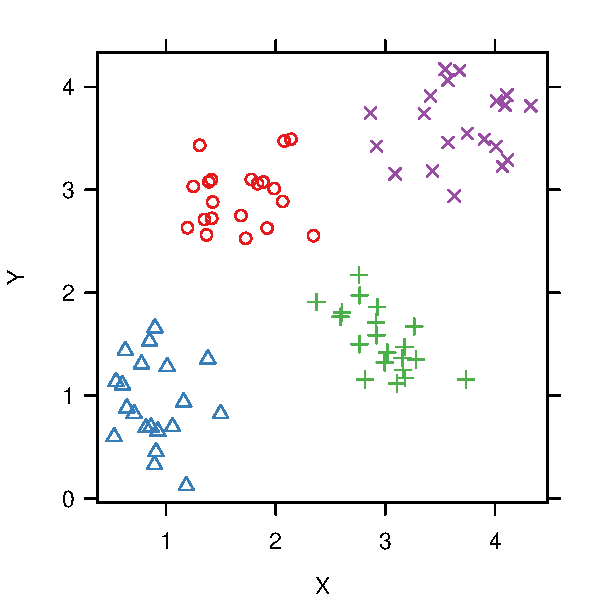
\includegraphics[width=\linewidth]{demo/elbow/correct-data.pdf}
  \end{minipage}
  \hspace{0.05in}
  \begin{minipage}{0.45\linewidth}
    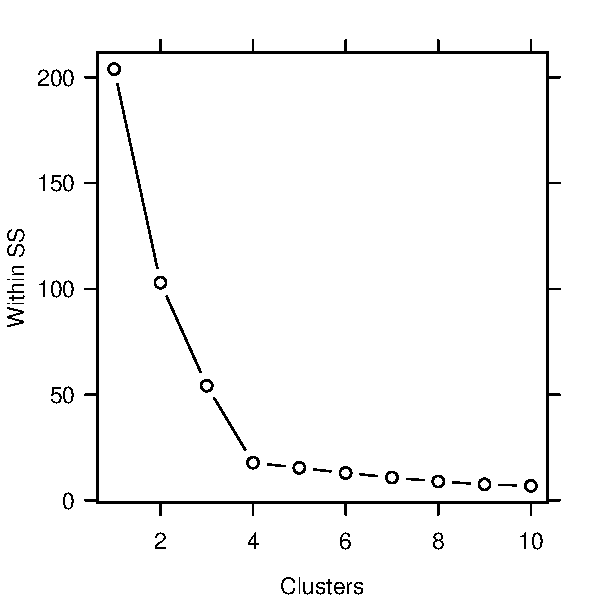
\includegraphics[width=\linewidth]{demo/elbow/correct-withinss.pdf}
  \end{minipage}
\end{minipage}
\begin{minipage}{\linewidth}
  \begin{minipage}{0.45\linewidth}
    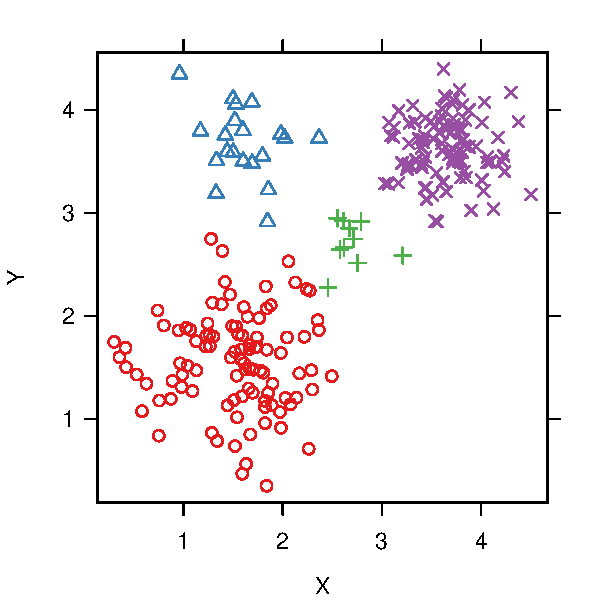
\includegraphics[width=\linewidth]{demo/elbow/incorrect-data.pdf}
  \end{minipage}
  \hspace{0.05in}
  \begin{minipage}{0.45\linewidth}
    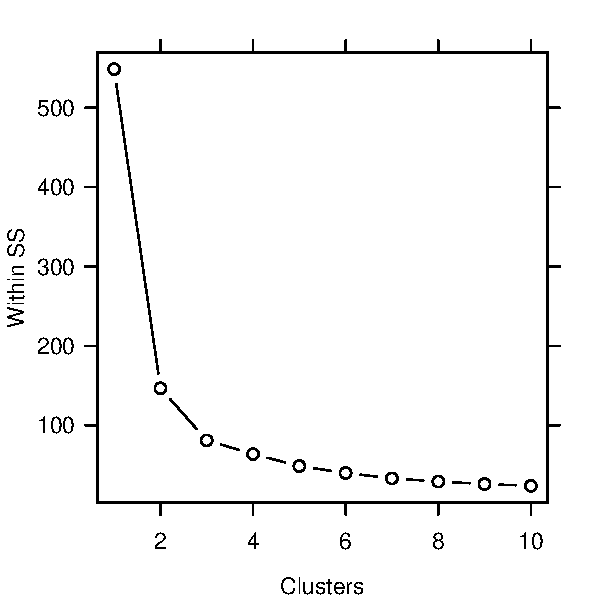
\includegraphics[width=\linewidth]{demo/elbow/incorrect-withinss.pdf}
  \end{minipage}
\end{minipage}
\caption{Left panels show the $(X,Y)$ data points; right panels
  show the corresponding values of the within-cluster sum of squares $W_k$
plotted against the number of clusters, $k$.}
\label{fig:elbow}
\end{figure}

Recently, there are several new proposals to find the $k$ automatically. Gap
statistics \citep{tibshirani2001estimating} estimates $k$ by comparing the
change in within-cluster dispersion with that expected under an appropriate
reference null distribution. Specifically, the graph of $\log(W_k)$ is
compared with its expectation under an appropriate null reference distribution
of the data. The value of $k$ associated with the largest gap between
$\log(W_k)$ and the reference curve is selected as optimal $k$.
\citet{sugar2003finding} proposed an approach which finds the number of
clusters based on distortion, a quantity that measures the average distance,
per dimension. It's backed by a rigorous theoretical justification based on
information-theoretic ideas.   \citet{fraley2002model}'s Model-based method
employs the EM algorithm to estimate the parameters in Gaussian mixture model,
and select the best model ($k$) using BIC criterion. Stability-based criterion
is also proposed to locate the best $k$ by some authors such as
\citet{ben2001stability}, \citet{wang2010consistent} and
\citet{fang2012selection}. \citet{chiang2010intelligent} provides a nice review
of existing methods for finding the right $k$ in published literature.

Most existing methods are either model based method requires strong modeling
assumptions or otherwise lack of clear interpretation and theoretical justification.
Although many view selecting the number of clusters as a model selection problem, very few
approaches this problem from the prediction point of view. Select model with
smallest prediction error via cross-validation is one of the simplest and most
widely used model selection techniques in supervised learning. The lack of
true class (label) in data set makes the adoption of cross-validation into
unsupervised learning problem difficult. A naive algorithm may works as following:
with the data split by rows into training set and test set, cluster the training 
data with parameter $k$; then predict each observation in test data by the closest
cluster center returned in last step. The prediction error is calculated by the 
difference between the predicted cluster centers and observations' true value, and algorithm 
picks the $k$ which minimizes such error. Such algorithm will always pick the maximum number 
of $k$ allowed because more cluster centers means more tight fit to the data space, therefore
smaller within-cluster dispersion even if the prediction is evaluated on an independent
test set \citep{hastie2009elements}.

One exception is \cite{tibshirani2005cluster}, which selects the optimal $k$ by prediction
strength. The strategy is to first cluster the test data and training data
into $k$ clusters respectively. Then, for each pair of observations that are
assigned to the same test cluster, algorithm determines whether they are also
assigned to the same cluster based on the training centers. The intuition here
is, if $k=k_0$, the true number of clusters, then the $k$ training set
clusters will be similar to the $k$ test clusters, and hence will predict them
well. However, a specifically defined prediction error measure is used in such
procedure, which is quite different from the one commonly used in
cross-validation procedure in supervised learning. \citet{wang2010consistent} also uses 
cross-validation to select the optimal $k$. Instead of selecting $k$ which minimizes 
prediction error, such method picks $k$ which minimizes the specifically defined 
clustering instability. Note that these methods minimize measures that are specifically defined,
which makes these methods hard to interpret or compare to other methods through analogy because
the underlying measures are unique and not well understood. 
 
The prediction error measure in our proposed method is exactly the same as in supervised learning.
Our method is a complete data-driven approach which doesn't rely on strong model assumption. Through novel form of partitioning data set, we effectively 
transferred an unsupervised learning problem into a supervised leaning problem, which is one of
the kind. By doing so, we are able to employing the cross-validation procedure in clustering 
a similar way as in supervised learning problem, so that much of the intuition from supervised learning
carries over. Hence, it's easy for reader to
understand the intuition behind our proposed method. Simulation and real data
application shows the superior performance of our proposed method compare with
existing methods in high-dimension settings and heavy-tailed data. Since the
embedded cross-validation procedure is well understood, it also makes our
method potentially easily to be extended in future study. 

Some proposed methods provide theoretical consistency result for choosing $k$. 
Assume data is a mixture of $G$ $p$-dimension clusters with equal prior, identically distributed with 
common covariance matrix and finite fourth moments in each dimension, \citet{sugar2003finding} shows
the Jump method will pick the correct $k$ under the conditions that cluster centers are sufficiently
separated and an appropriate transformation is used. Specifically, let $\Delta\sqrt{p}$ denotes the 
minimum Euclidean distance between cluster centers, \citet{sugar2003finding} shows that the jump will
be maximized at $k=G$ given that $\Delta > 6$ and the existence of a positive $Y$ such that
\[	\left(\frac{p\Delta^2W}{9G}\right)^{-Y}+\left(W\left[\frac{2^{2H^*(X)}}{K^2_{max}2\pi e}\right]-(\frac{\Delta}{6})^2(1-W) \right)^{-Y} < 2	\]
and $\left(\frac{p\Delta^2W}{9G}\right)^{-Y} <1/2$, where $H^*(X)$ is the minimum entropy of the cluster 
membership over each dimension and $W =1- \frac{6^4V_{\mathbf{X}}}{(\Delta^2-36)^2}$ with $V_{\mathbf{X}} = var\left( 1/p ||\mathbf{X}-\mu_j||^2_{\Gamma^{-1}} \mid \mathbf{X} \hspace{0.05in}\text{in jth cluster}\right)$

\cite{tibshirani2005cluster} proved that the prediction strength method is consistent under the setting 
that the observations in $p$-dimension are uniformly distributed within one unit from their respective cluster centers, with minimum distance between the $G$ cluster centers is four unit. Under such well-separated setting, 
they show that 
\[ ps(G) = 1+ o_p(1), \hspace{0.5in} \underset{k \geq G+1}{\text{sup}} ps(k)\leq \frac{2}{3}+ o_p(1) \]
therefore $\hat{k}$ is consistent in estimating $G$.  
When data does come from mixture of Gaussian distribution, the model-based method of \citet{fraley2002model} is consistent in estimating $k$ in low dimension.

Let $\Psi$ denotes any given base-clustering algorithm (e.g $k$-means), and $\Psi(Z,k)$ the clustering obtained by applying $\Psi$ on data $Z$ with parameter $k$. Also let $k_0$ be the optimal number of cluster and $d\{\Psi(Z_1,k),\Psi(Z_2,k)\}$ be the measure of distance between clustering $\Psi(Z_1,k)$ and $\Psi(Z_2,k)$ where $Z_1$ and $Z_2$ are two independent samples from population. \citet{wang2010consistent} shows that their proposed method will consistently select $k = k_0$, given such $k_0$ exists and $d\{\Psi(Z_1,k),\Psi(Z_2,k)\}$ converges to zero at proper rate $r_k$. However, $k_0$ is defined as the most stable number for $\Psi$ among all the possible $k$, instead of the number of components in mixture model or well-separated compact regions commonly seen in literature. Therefore, their consistent result actually is convergent result, i.e. the selected $k$ converges to its limit $k_0$ given such limit exists.

\section{Cross-validation for selecting the number of clusters}
\label{sec:meth}
Cross-validation is commonly used for model selection in supervised learning
problems.  In these settings, the data comes in the form of $N$
predictor-response pairs, $(X_1, Y_1), \dotsc, (X_N, Y_N)$, with $X_i \in
\R^{p}$ and $Y_i \in \R^{q}$.  The data can be represented as a matrix with
$N$ rows and $p + q$ columns.  We partition the data into $K$ hold-out
``test'' subsets, with $K$ typically chosen to be $5$ or $10$.  For each
``fold'' $r$ in the range $1, \dotsc, K$, we permute the rows of the data
matrix to get $\dataX$, a matrix with the $r$th test subset as its trailing
rows.  We partition $\dataX$ as
\[
  \dataX =
  \begin{bmatrix}
    \Xtrain & \Ytrain \\
    \Xtest  & \Ytest
  \end{bmatrix}.
\]
We use the training rows $[ \Xtrain\ \Ytrain ]$ to fit a regression model
$\hat Y = \hat Y(X)$, and then evaluate the performance of this model on the
test set, computing the cross-validation error $\|\Ytest - \hat Y(\Xtest)\|^2$
or some variant thereof.  We choose the model with the smallest
cross-validation error, averaged over all $K$ folds.

In unsupervised learning problems like factor analysis and clustering, the
features of the observations are not naturally partitioned into ``predictors''
and ``responses'', so we cannot directly apply the cross-validation procedure
described above.  For factor analysis, there are at least two versions of
cross-validation.  \citet{wold78cross} proposed a ``speckled'' holdout, where
in each fold we leave out a subset of the elements of the data matrix.  Wold's
procedure works well empirically, but does not have any theoretical support,
and it requires a factor analysis procedure that can handle missing data.
\citet{owen2009bi} proposed a scheme called ``bi-cross-validation'' wherein
each fold designates a subset of the data matrix columns to be response and a
subset of the rows to be test data.  This generalized a procedure due to
\citet{gabriel2002biblot}, who proposed holding out a single column and a
single row at each fold.  Owen and Perry proved that this procedure is
self-consistent, in the sense that it performs the correct model selection in
the absence of noise, and \citet{perry2009cross} provided more theoretical
support.

In this report, we extend the Wold and Gabriel methods to the clustering
problem, specifically to choose an appropriate number of clusters for a
dataset.  We prove that the Gabriel method is self-consistent, and we analyze
some of its properties in the presence of noise.  We compare these methods to
state-of-the-art algorithms, and show that both are competitive.

%% [POP] This paragraph doesn't fit into the section.  Maybe put it in the introduction?
%% 
%% Cross-Validation technique, one of the most commonly used and popular model
%% selecting method in supervised learning, can not be used naively in
%% unsupervised learning context. Since prediction error of new observation is
%% calculated by its distance to the nearest cluster center, more cluster centers
%% means much tighter fit to the feature space, and hence smaller distance
%% (prediction error) of observation to its nearest cluster center. This holds
%% even when the prediction is evaluated on an independent test set
%% \citep{hastie2009elements}. Therefore, CV prefers larger $k$ if we do the CV
%% naively.

We now give the details of how to implement
the Gabriel cross-validation to locate the optimal cluster number $k$. The
Wold cross-validation algorithm is described in Appendix $A$.

\subsection{Gabriel CV algorithm}
\label{sec:gabriel-cv-algorithm}
We are given a data matrix with $N$ rows and $P$ columns.  In each fold of
cross-validation, we permute the rows and columns of the data matrix and then
partition the rows and columns as $N = n + m$ and $P = p + q$ for 
non-negative integers $n$, $m$, $p$, and $q$.  We treat the first $p$
columns as ``predictors'' and the last $q$ columns as ``responses'';
similarly, we treat the first $n$ rows as ``training'' and the last $m$ rows
as ``test''.  In block form, the permuted data matrix is
\[
  \dataX
  =
  \begin{bmatrix}
    \Xtrain & \Ytrain \\
    \Xtest  & \Ytest
  \end{bmatrix},
\]
where
$\Xtrain \in \R^{n \times p}$,
$\Ytrain \in \R^{n \times q}$,
$\Xtest \in  \R^{m \times p}$,
and
$\Ytest \in  \R^{m \times q}$.

Given such a partition of $\dataX$, we perform four steps for each value of
$k$, the number of clusters:
\begin{enumerate}
  \item \label{step:gabriel-cluster}
    \textbf{Cluster:}
    Cluster $Y_{1}, \dotsc, Y_n$, the rows of $\Ytrain$, yielding the
    assignment rule $\hGY : \R^q \to \{ 1, \dotsc, k \}$ and the
    cluster means $\bmuY_1, \dotsc, \bmuY_k$.  Set $\hGY_i = \hGY(Y_i)$ to
    be the assigned cluster for row $i$.
  \item \label{step:gabriel-classify}
    \textbf{Classify:}
    Take $X_{1}, \dotsc, X_n$, the rows of $\Xtrain$ to be predictors,
    and take $\hGY_1, \dotsc, \hGY_n$ to be corresponding class labels.  Use
    the pairs $\{ (X_i, \hGY_i) \}_{i=1}^{n}$ to train a classifier
    $\hGX : \R^p \to \{ 1, \dotsc, k \}$.
  \item \label{step:gabriel-predict}
    \textbf{Predict:}
    Apply the classifier to $X_{n+1}, \dotsc, X_{n+m}$, the rows of
    $\Xtest$, yielding predicted classes $\hGX_i = \hGX(X_i)$ for
    $i = n+1, \dotsc, n+m$.  For each value of $i$ in this range, compute
    predicted response $\hat Y_i = \bmuY(\hGX_i)$, where
    $\bmuY(g) = \bmuY_g$.
  \item \label{step:gabriel-evaluate}
    \textbf{Evaluate:}
    Compute the cross-validation error
    \[
      \CV(k) = \frac{1}{m} \sum_{i=n+1}^{n+m} \|Y_i - \hat Y_i\|^2,
    \]
    where $Y_{n+1}, \dotsc, Y_{n+m}$ are the rows of $\Ytest$.
\end{enumerate}
\noindent
In principle, we could use any clustering and classification methods in
steps~\ref{step:gabriel-cluster} and~\ref{step:gabriel-classify}.  In this
report, we use $k$-means as the clustering algorithm.  For the classification
step, we compute the mean value of $X$ for each class; we assign an
observation to class $g$ if that class has the closest mean (randomly breaking
ties between classes).  The classification step is equivalent to linear
discriminant analysis with equal class priors and identity noise covariance
matrix.

To choose the folds, we randomly partition the rows and columns into $K$ and
$L$ subsets, respectively.  Each fold is indexed by a pair $(r,s)$ of
integers, with $r \in \{1, \dotsc, K\}$ and $s \in \{1, \dotsc, L\}$.  Fold
$(r,s)$ treats the $r$th row subset as ``test'', and the $s$th column subset
as ``response''.  We typically take $K = 5$ and $L = 2$.  For the number of
clusters, we select the value of $k$ that minimizes the average of $\CV(k)$
over all $K \times L$ folds (choosing the smallest value of $k$ in the event
of a tie).
%------------------------------------------------------------------
\section{Self-Consistency of Gabriel CV method}

This section gives the self-consistency proof of the proposed Gabriel method.
Specifically, we will show that under appropriate conditions, in the absence
of noise, the Gabriel cross-validation procedure finds the optimal number of
clusters.


Because $k$-means algorithm is essential to the method, we review the
procedure here.  Given a set of observations $\{ x_1, \dotsc ,x_n \}$, and a
specified the number of clusters $k$, the goal of the $k$-means procedure is
to find a set of $k$ or cluster centers $A = \{ a_1, \dotsc, a_k \} $
minimizing the within cluster dispersion
\[
  W(A) = \sum_{i=1}^{n} \min_{a \in A} \|x_i - a\|^2.
\]
This implicitly defines a cluster assignment rule
\[
  g(x) = \argmin_{g \in \{1, \dotsc, k\}} \|x - a_g\|^2,
\]
with ties broken arbitrarily.  We will assume that the $k$-means procedure
finds an optimal solution, $A$, but we will not assume that this solution is
unique.


It will suffice to analyze a single fold of the cross-validation procedure.
As in in section~\ref{sec:gabriel-cv-algorithm} we assume that the $P$
variables of the data set have been partitioned into $p$ predictor variables
represented in vector~$X$ and $q$ response variables represented in
vector~$Y$.  The $N$ observations have been divided into two sets: $n$ train
observations and $m$ test observations.  The following theorem gives
conditions for Gabriel CV to recover the true number of clusters in the
absence of noise.


\begin{theorem}\label{thm:self-consistency}

Let $\{ (X_i, Y_i) \}_{i=1}^{n+m}$ be the data from a single fold of Gabriel
cross-validation.  For any $k$, let $CV(k)$ be the cross-validation error for
this fold, computed as described in Section~\ref{sec:gabriel-cv-algorithm}.
We will assume that there are $K$ true centers $\mu(1), \dotsc,\mu(K)$, with
the $g$th cluster center partitioned as $\mu(g) = \bigl(\muX(g),
\muY(g)\bigr)$ for $g = 1, \dotsc, K$.  Suppose that
\begin{enumerate}[label=(\roman*)]
  \item \label{asn:self-consistency-noiseless}
    Each observation $i$ has a true cluster $G_i \in \{ 1, \dotsc, K \}$.
    There is no noise, so that $X_i = \muX({G_i})$ and $Y_i = \muY(G_i)$ for
    $i = 1, \dotsc, n+m$.
  \item \label{asn:self-consistency-distinct-mux}
    The vectors $\muX(1), \dotsc,\muX(K)$ are all distinct.
  \item \label{asn:self-consistency-distinct-muy}
    The vectors $\muY(1), \dotsc,\muY(K)$ are all distinct.
  \item \label{asn:self-consistency-train}
    The training set contains at least one member of each cluster: for all $g$
    in the range $1, \dotsc, K$, there exists at least one $i$ in the range
    $1, \dotsc, n$ such that $G_i = g$.
  \item \label{asn:self-consistency-test}
    The test set contains at least one member of each cluster: for all $g$ in
    the range $1, \dotsc, K$, there exists at least one $i$ in the range $n+1,
    \dotsc, n+m$ such that $G_i = g$.
\end{enumerate}
Then $CV(k) < CV(K)$ for $k < K$, and $CV(k) = CV(K)$ for $k > K$, so that
Gabriel CV correctly chooses $k = K$.
\end{theorem}

This theorem is implied by the following two lemmas.

\begin{lemma}
Suppose that the assumptions of Theorem~\ref{thm:self-consistency} are in
force.  If $k < K$, then $\CV(k) > 0$.
\end{lemma}
\begin{proof}
By definition,
\[
  \CV(k)
    =
      \sum_{i=n+1}^{n+m}
        \| Y_i - \bmuY (\hGX_i) \|^2,
\]
where $\bmuY(g)$ is the center of cluster $g$ returned from applying $k$-means
to $Y_1, \dotsc, Y_n$.  Assumptions~\ref{asn:self-consistency-noiseless}
and~\ref{asn:self-consistency-test}, imply that as $i$ ranges over the test
set $n+1, \dotsc, n+m$, the response $Y_i$ ranges over all distinct values in
$\{ \muY(1), \dotsc, \muY(K) \}$.
Assumption~\ref{asn:self-consistency-distinct-muy} implies that there are
exactly $K$ such distinct values.  However, there are only $k$ distinct values
of $\bmuY(g)$.  Thus, at least one summand
\(
  \| Y_i - \bmuY(\hGX_i) \|^2
\)
is nonzero.  Therefore,
\(
  \CV(k) > 0.
\)
\end{proof}

\begin{lemma}
Suppose that the assumptions of Theorem~\ref{thm:self-consistency} are in
force.  If $k \geq K$, then $\CV(k) = 0$.
\end{lemma}
\begin{proof}
From assumptions~\ref{asn:self-consistency-noiseless},
\ref{asn:self-consistency-distinct-muy},
and~\ref{asn:self-consistency-train}, we know the cluster centers
gotten from applying $k$-means to $Y_1, \dotsc, Y_n$ must include
$\muY(1), \dotsc, \muY(K)$.  Without loss of generality, suppose that
$\bmuY(g) = \muY(g)$ for $g = 1, \dotsc, K$.  This implies that
$\hGY_i = G_i$ for $i = 1, \dotsc, n$.  Thus, employing
assumption~\ref{asn:self-consistency-noiseless} again, we get that
$\bmuX(g) = \muX(g)$ for $g = 1, \dotsc, K$.


Since assumption~\ref{asn:self-consistency-distinct-mux} ensures that
$\muX(1), \dotsc, \muX(K)$ are all distinct, we must have that $\hGX_i = G_i$
for all $i = 1, \dotsc, m+n$.  In particular, this implies that $\bmuY(\hGX_i)
= Y_i$ for $i = 1, \dotsc, m+n$, so that $\CV(k) = 0$.
\end{proof}
%-------------------------------------------------------------
\section{Analysis of Gabriel Cross-Validation with Gaussian Noise}

\subsection{Single Cluster}
Now we we analyze the asymptotic performance of Gabriel Cross-Validation, in
the case of Gaussian noise. Our main result is that with single-cluster
Gaussian data, if the predictor and response columns of $\dataX$ are weakly
correlated or independent, then the method will correctly prefer $k = 1$ to
$k = 2$ clusters. We first state the result in the case where $\dataX$ has two 
columns, and later generalize this result to higher dimensions.

\begin{proposition}
Suppose that $\{ (X_i, Y_i) \}_{i=1}^{n + m}$ is data from a single fold
of Gabriel cross-validation, where each $(X,Y)$ pair in $\R^2$ is an
independent draw from a mean-zero multivariate normal distribution with unit
marginal variances and correlation $\rho$.  In this case, the data are drawn
from a single cluster; the true number of clusters is~$1$.  If $|\rho| < 0.5$,
then $\CV(1) < \CV(2)$ with probability tending to one as $m$ and $n$ increase.
\end{proposition}

\begin{proof}
Given $(X_1, Y_1), \dotsc, (X_n, Y_n)$, we first apply $k$-means to $\{ Y_i
\}_{i=1}^{n}$. With $k = 1$, the single-cluster centroid will
be equal to $\bar Y_n$, the sample mean of the $Y_1, \dotsc, Y_n$, approximately equal to
$\E(Y) = 0$, with error of size $\OhP(n^{-1/2})$. The cross-validation error
will be
\[
  \CV(1) = \frac{1}{m} \sum_{i=n+1}^{n+m} \| Y_i - \bar Y_n \|^2
         = 1 + \OhP(m^{-1/2}) + \OhP(n^{-1/2}).
\]

Now we will consider the $k = 2$ case.  If $n$ is large enough, then
\citet{pollard1981strong} showed that the centroids $\bmuY_1$ and $\bmuY_2$
will be close to $\E(Y \mid Y > 0) = \sqrt{2/\pi}$ and $\E(Y \mid Y < 0) =
-\sqrt{2/\pi}$.  We have used Lemma~\ref{lem:truncated-normal-moments}
(Appendix~\ref{app:technical-lemmas}) to compute the expectations.  Further,
\citet{pollard1982central} showed that the errors will be of size $\OhP(n^{-1/2})$.

If $\rho > 0$ and $n$ is large enough, then classification rule learned from
$\{(X_i, \hGY_i)\}_{i=1}^{n}$ variables will be determined according to
whether $X > 0$; if $\rho < 0$ then the decision is according to whether $X <
0$.  More specifically, the decision boundary will be at $0 + \OhP(n^{-1/2})$.

In the $\rho > 0$ case, the cross-validation error will be
\begin{align*}
  \CV(2)
  &=
    \frac{1}{m}
    \sum_{i=n+1}^{n+m}
      \| (Y_i - \bmuY_1) 1\{\hGX_i = 1\} \|^2
      +
      \| (Y_i - \bmuY_2) 1\{\hGX_i = 2\} \|^2
\\
  &=
    \E[(Y - a)^2 1\{ X > 0\}] + \E[(Y + a)^2 1\{X < 0\}]
      + \OhP(m^{-1/2}) + \OhP(n^{-1/2}),
\end{align*}
where $a = \sqrt{2/\pi}$.  From the joint normality of $X$ and $Y$, it follows
that $Y \mid X$ is normal with mean $\rho X$ and variance $(1 - \rho^2)$, so
that $\E[(Y - a)^2 \mid X] = (\rho X - a)^2 + (1 - \rho^2)$.  Applying
Lemma~\ref{lem:truncated-normal-moments}, we get that for large $m$ and $n$,
the Gabriel cross-validation error is close to
$1 + a^2 (1 - 2 \rho)$.  

In the $\rho < 0$ case, a similar calculation shows that $\CV(2)$ is close to
$1 + a^2 (1 + 2 \rho)$.  In particular, if $|\rho| < 0.5$, then with
probability tending to $1$ and $m$ and $n$ increase, the asymptotic
cross-validation error for $k = 1$ will be smaller than for $k = 2$.
\end{proof}

We confirm this result with a simulation.  We perform $10$ replicates.  In each
replicate, we generate $20000$ observations from a mean-zero bivariate normal
distribution with unit marginal variances and correlation $\rho$.  We perform
a single $2 \times 2$ fold of Gabriel cross-validation and report the
cross-validation mean squared error for the number of clusters $k$ ranging
from $1$ to $5$.  Figure~\ref{fig:nullcorr-equal} shows the cross-validation
errors for all $10$ replicates.  The simulation demonstrates that in the
Gabriel cross-validation criterion chooses the correct answer $k = 1$ whenever
$\rho < 0.5$; the criterion chooses $k = 2$ clusters whenever $|\rho| > 0.5$.

\begin{figure}[H]
\centering
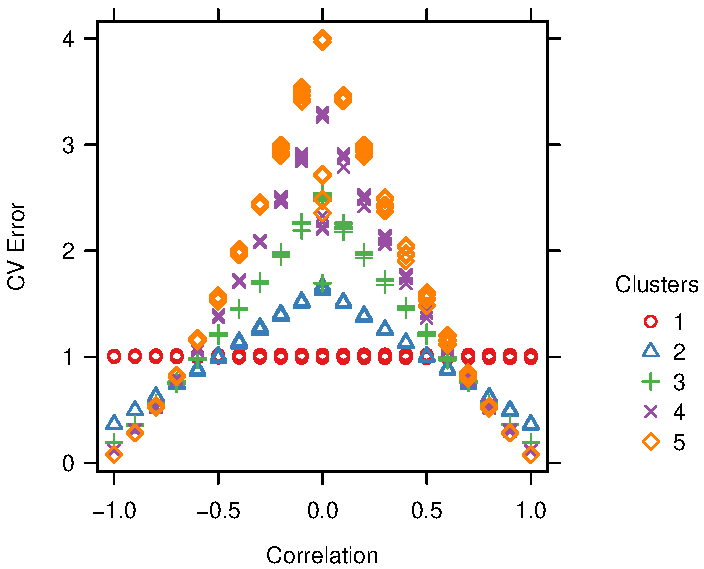
\includegraphics[width=3in]{demo/nullcorr/equal.pdf}
\caption{Cross-validation error on $10$ replicates, with the number of
clusters $k$ ranging from $1$ to $5$.  Data is generated from two-dimensional
multivariate normal distribution with correlation $\rho$.  The Gabriel
cross-validation criterion chooses the correct answer $k = 1$ whenever
$\rho < 0.5$; the criterion chooses $k = 2$ clusters whenever $|\rho| > 0.5$.}
\label{fig:nullcorr-equal}
\end{figure}

The reason why Gabriel CV method tends to select larger $k$ when correlation is high 
between dimensions is that it resembles the naive method mentioned in section \ref{sec:intro} 
under such circumstance. In fact, if $X$, $Y$ are perfectly correlated, Gabriel method is 
equivalent to the naive method.

Proposition $1$ gives a very simple condition for the Gabriel method to correctly 
pick $k=1$ with single cluster in $2$ dimensions. The following proposition generalizes
such condition for data in arbitrary dimension. 

\begin{proposition}
Suppose that $\{ (X_i, Y_i) \}_{i=1}^{n + m}$ is data from a single fold
of Gabriel cross-validation, where each $(X,Y)$ pair in $\R^{p+q}$ is an
independent draw from a mean-zero multivariate normal distribution with 
covariance matrix $\Sigma_{XY}= \left( \begin{smallmatrix} \Sigma_{XX} & \Sigma_{XY} \\ 
 \Sigma_{YX} & \Sigma_{YY} \end{smallmatrix}\right)$, with $\Sigma_{YY}$ has leading 
eigenvalue $\lambda_1$ and corresponding eigenvector $u_1$. In this case, the data are drawn
from a single cluster; the true number of clusters is~$1$.  If  $\frac{\sqrt{\lambda_1}}{2}
 > \frac{u^T_1\Sigma_{YX}\Sigma_{XY}u_1}{\sqrt{u^T_1\Sigma_{YX} \Sigma_{XX} \Sigma_{XY} u_1}}$,
then $\CV(1) < \CV(2)$ with probability tending to one as $m$ and $n$ increase.
\end{proposition}

\begin{proof}
Let $X$ and $Y$ be jointly multivariate normal distributed with mean $\mathbf{0}$ and covariance matrix $\Sigma_{XY}$, i.e.
\[	(X,Y) \sim \mathcal{N} \left( \mathbf{0}, \Sigma_{XY}\right)	\]
where $\Sigma_{XY}=\begin{bmatrix} \Sigma_{XX} & \Sigma_{XY} \\  \Sigma_{YX} & \Sigma_{YY} \end{bmatrix}$.

Let $\Sigma_{YY} = U \Lambda U^T$  be the eigendecomposition of $\Sigma_{YY}$, with leading eigenvalue $\lambda_1$ and corresponding eigenvector $u_1$. Then the centroid of $k$-means applying on $(y_1,..,y_n)$ is on the first PC 
of $Y$,\[	E(u^T_1 Y|u^T_1 Y>0) = \bar{\mu}^Y_1 =\sqrt{2 \lambda_1/\pi}u_1\] and 
\[	E(u^T_1 Y|u^T_1 Y<0) = \bar{\mu}^Y_2 =-\sqrt{2 \lambda_1/\pi}u_1\]
 where $u^T_1 Y \sim \mathcal{N}(0,\lambda_1)$.

To compute $\bar{\mu}^X_1 = E(X|u^T_1 Y>0)$, we need to know the conditional distribution $X|u^T_1 Y$. Since $(X,Y)$ has multivariate normal distribution, $(X,u^T_1 Y)$ also has a multivariate normal distribution with mean $\mathbf{0}$ and covariance matrix
$$\Sigma_{X,u^T_1 Y}=\begin{bmatrix} \Sigma_{XX} & \Sigma_{XY} u_1 \\  u^T_1 \Sigma_{YX} & \lambda_1 \end{bmatrix}$$
The conditional distribution $X|u^T_1 Y$ is hence normal with mean
 $$\mu_{X|u^T_1 Y} = \Sigma_{XY} u_1 \lambda^{-1}_1 u^T_1 Y $$
Therefore, 
\begin{align}
\bar{\mu}^X_1 &= E(X \mid u^T_1 Y>0) \nonumber \\ \nonumber
 			  &= E\left(E[X \mid u^T_1 Y] \mid u^T_1 Y>0\right) \\ \nonumber
 			  &=  E\left(\Sigma_{XY} u_1 \lambda^{-1}_1 u^T_1 Y \mid u^T_1 Y>0\right)\\ \nonumber
 			  &= \lambda^{-1}_1 \Sigma_{XY}u_1 E(u^T_1 Y \mid u^T_1 Y>0) \\ \nonumber
 			  &= \lambda^{-1}_1 \Sigma_{XY}u_1 \sqrt{2 \lambda_1/\pi} \\ \nonumber
 			  &= \sqrt{2 / \lambda_1 \pi} \Sigma_{XY}u_1
\end{align}
Similar calculation yields $\bar{\mu}^X_2 = -\sqrt{2 / \lambda_1 \pi} \Sigma_{XY}u_1$.
The decision rule to classify any observed value of $X$ to $\bar{\mu}^X_1$ is therefore
\[	(\bar{\mu}^X_1)^T X >0	\hspace{0.2in}\text{or} \hspace{0.2in} u^T_1\Sigma_{YX}X>0\] 
Since $u^T_1\Sigma_{YX}X$ is a linear combination of $X$, it also has normal distribution 
\[	\mathcal{N} \left( 0, u^T_1\Sigma_{YX} \Sigma_{XX} \Sigma_{XY} u_1\right)	\]
And $(Y,u^T_1\Sigma_{YX}X)$ also have multivariate normal distribution with mean $\mathbf{0}$ 
and covariance matrix
\[
\begin{bmatrix}
\Sigma_{YY} & \Sigma_{YX}\Sigma_{XY}u_1  \\
u^T_1\Sigma_{YX}\Sigma_{XY} &  u^T_1\Sigma_{YX} \Sigma_{XX} \Sigma_{XY} u_1
\end{bmatrix}
\]
The conditional distribution of $Y|u^T_1\Sigma_{YX}X$ is also multivariate normal with mean 
\[	
\mu_{Y|u^T_1\Sigma_{YX}X } = \Sigma_{YX}\Sigma_{XY}u_1 (u^T_1\Sigma_{YX} \Sigma_{XX} \Sigma_{XY} u_1)^{-1}u^T_1\Sigma_{YX}X	
\]
The $Y$ center for $u^T_1\Sigma_{YX}X>0$ is
\begin{align}
\hat{\mu}^Y_1 &= E(Y|u^T_1\Sigma_{YX}X>0) \nonumber \\ \nonumber
 		      & =  \Sigma_{YX}\Sigma_{XY}u_1 (u^T_1\Sigma_{YX} \Sigma_{XX} \Sigma_{XY} u_1)^{-1} E(u^T_1\Sigma_{YX}X \mid u^T_1\Sigma_{YX}X>0) \\ \nonumber
\end{align}
Note that $u^T_1\Sigma_{YX}X$ has normal distribution $\mathcal{N} \left( 0, u^T_1\Sigma_{YX} \Sigma_{XX} \Sigma_{XY} u_1\right)$, so
\[
E(u^T_1\Sigma_{YX}X \mid u^T_1\Sigma_{YX}X>0) = \sqrt{2/\pi}\cdot\sqrt{u^T_1\Sigma_{YX} \Sigma_{XX} \Sigma_{XY} u_1}
\]
Therefore, we have the $Y$ center for $u^T_1\Sigma_{YX}X>0$ be
\begin{align*}
\hat{\mu}^Y_1 &= \sqrt{2/\pi}\cdot\sqrt{u^T_1\Sigma_{YX} \Sigma_{XX} \Sigma_{XY} u_1} \hspace{0.1in} \Sigma_{YX}\Sigma_{XY}u_1 (u^T_1\Sigma_{YX} \Sigma_{XX} \Sigma_{XY} u_1)^{-1} \\
&=\frac{\sqrt{2/\pi}}{\sqrt{u^T_1\Sigma_{YX} \Sigma_{XX} \Sigma_{XY} u_1}} \Sigma_{YX}\Sigma_{XY}u_1
\end{align*} 
 
Recall that $\bar{\mu}^Y_1 =\sqrt{2 \lambda_1/\pi}u_1$, to judge if $CV(2) > CV(1)$, one only need to compare the distance between  $\hat{\mu}^Y_1$  and  $\bar{\mu}^Y_1$ with distance between  $\hat{\mu}^Y_1$ and grand mean $0$. By variance and bias decomposition of prediction MSE, when variance is the same, only bias influence the MSE. 

After some linear algebra manipulation, we get
$||\hat{\mu}^Y_1 - \bar{\mu}^Y_1||^2 > ||\hat{\mu}^Y_1||^2$ or $CV(2) > CV(1)$ iff
\[
 \frac{\sqrt{\lambda_1}}{2} > \frac{u^T_1\Sigma_{YX}\Sigma_{XY}u_1}{\sqrt{u^T_1\Sigma_{YX} \Sigma_{XX} \Sigma_{XY} u_1}} 
\]
\end{proof}

Above equation gives the condition of when Gabriel CV method would correctly choose $k=1$ over $k=2$. Although the expression is succinct, it's not straight forward to see how the structure of covariance matrix $\Sigma_{XY} \in \mathbb{R}^{(p+q) \times (p+q)}$ affects the performance of Gabriel CV method. Here, assuming covariance matrix has compound symmetric structure where only the matrix dimension $p+q$ and $\rho$ are variables, i.e. $$\Sigma_{XY} = \begin{pmatrix}
1 & \rho & \cdots & \rho \\
\rho & 1 & \cdots & \rho \\
\vdots & \vdots & \cdots & \rho \\
\rho& \rho & \cdots & 1 \\
\end{pmatrix}
$$
we are able to feel what above equation implies for this specific case. Another reason to use the compound symmetric structure covariance matrix is that it's invariant under the permutation of each column vector in the matrix. Given that Gabriel CV method randomly choose $p$ columns as $X$ ($q$ columns as $Y$), compound symmetric structure insures that the covariance matrix $\Sigma_{XY}$ always look the same no matter which $p$ columns selected as $X$.  

If we do $2$ fold cross-validation in the column, i.e. $p=q$, then the result in Proposition $2$ implies that the boundary value of $\rho$ is 
\[
	\rho^* = \frac{1}{p+1}
\]
under the compound symmetric structure given above, where $\Sigma_{XY}$ has $p+q=2p$ dimension. If $\rho < \rho^*$, then Gabriel CV prefers $CV(1)$ over $CV(2)$ and vice versa. It means the boundary value $\rho^*$ depends on the dimension of $\Sigma_{XY}$ linearly. 

If dimension is $p+q = 2$ with $p=q$, then above boundary condition shows the boundary value $\rho^* = 0.5$, while for dimension $p+q = 100$, the  boundary value $\rho^* = \frac{1}{51}$. However, such value also depends on the ratio of $p$ over $q$. Also in $p+q = 100$ dimension, if we pick $p=2$ and $q=98$ (leave majority of the columns for clustering), the the boundary value $\rho^* \in (\frac{1}{6},\frac{1}{7})$. 

\begin{theorem}
Suppose that $\{ (X_i, Y_i) \}_{i=1}^{n + m}$ is data from a single fold
of Gabriel cross-validation, where each $(X,Y)$ pair in $\R^2$ is an
independent draw from a mean-zero multivariate normal distribution with unit
marginal variances and correlation $\rho$.  In this case, the data are drawn
from a single cluster; the true number of clusters is~$1$.  If $|\rho| < 0.5$,
then $\CV(1) < \CV(k)$, $k > 1$ with probability tending to one as $m$ and $n$ increase.
\end{theorem}

\begin{proof}
Given $(X_1, Y_1), \dotsc, (X_n, Y_n)$, let $A_k = \{a_1,a_2,...,a_k\}$ denotes the set of cluster centers from applying $k$-means to $\{ Y_i\}_{i=1}^{n}$ with parameter $k$. Because $\{ Y_i\}_{i=1}^{n}$ is symmetric, it's easy to see that the cluster centers are symmetric around $0$, i.e. if $a^* \in A_k$ then $-a^* \in A_k$. The $k$ clusters are symmetric in the same sense. Also, if $k$ is odd, then only one cluster contains both negative and positive $Y$ and it's symmetric with center $0$. The rest have pure positive or negative intervals; if $k$ is even, then all clusters have pure positive or negative intervals. 

Let $a_i$ denotes a cluster center with interval $[b_i, c_i]$. By above argument, either $0 \leq b_i < c_i$ ($b_i < c_i \leq 0$) or $b_i = -c_i$ which corresponding to $a_i=0$ with $k$ be odd. By symmetry, it's sufficient to only consider case $0 \leq b_i < c_i$ (with $a_i > 0 $) and $b_i = -c_i$ (with $a_i = 0 $) with $\rho \geq 0$. 

From joint normality of $X$ and $Y$, it follows that $X \mid Y$ is normal with mean $\rho Y$. Therefore, the mean value $\bar{X}_i$ of $X$ in cluster with $Y$ center $a_i$ is  

\begin{align*}
	\bar{X}_i &= E[X \mid b_i \leq Y \leq c_i] \\
			&= E[ E(X \mid Y) \mid b_i \leq Y \leq c_i] \\
			&= E[\rho Y \mid b_i \leq Y \leq c_i] \\
			&= \rho E[ Y \mid b_i \leq Y \leq c_i] \\
			&= \rho a_i
\end{align*}

That is, the mean values of $X$ in the $k$ clusters is $\{\rho a_1,\rho a_2,...,\rho a_k\}$. Because we assign each observation to the closest $\bar{X}_i$, $i=1,2,...,k$, it's easy to see the corresponding interval on $X$ for $\bar{X}_i = \rho a_i$ is $[\frac{\rho \left( a_{i-1}+a_i\right)}{2}, \frac{\rho \left( a_{i}+a_{i+1}\right)}{2}]$, where $a_{i-1}$ and $a_{i+1}$ are the two adjacent centers to $a_i$ on $Y$. Note that $[\frac{ \left( a_{i-1}+a_i\right)}{2}, \frac{\left( a_{i}+a_{i+1}\right)}{2}] = [b_i, c_i]$ by the algorithm definition of $k$-means. The $Y$ center for such interval on $X$ is

\begin{align*}
	\hat{\mu}^Y_i &= E[Y \mid \frac{\rho \left( a_{i-1}+a_i\right)}{2} \leq X \leq \frac{\rho \left( a_{i}+a_{i+1}\right)}{2}] \\
	 &= E[ E(Y \mid X) \mid \frac{\rho \left( a_{i-1}+a_i\right)}{2} \leq X \leq \frac{\rho \left( a_{i}+a_{i+1}\right)}{2}] \\
	 &= E[ \rho X \mid \frac{\rho \left( a_{i-1}+a_i\right)}{2} \leq X \leq \frac{\rho \left( a_{i}+a_{i+1}\right)}{2}] \\
	 & =  \rho E[X \mid \frac{\rho \left( a_{i-1}+a_i\right)}{2} \leq X \leq \frac{\rho \left( a_{i}+a_{i+1}\right)}{2}] \\
	  & =  \rho E[X \mid \rho b_i \leq X \leq \rho c_i] \\
	  &\leq \rho a_i
\end{align*}

where the equality holds if $b_i = -c_i$ or $\rho = 1$ on the last step. This is because 

\begin{align*}
	 E[X \mid \rho b_i \leq X \leq \rho c_i] &= E[Y \mid \rho b_i \leq Y \leq \rho c_i] \\
	\mathtt{0 \leq b_i < c_i}, \hspace{0.05in} \mathtt{0 \leq \rho \leq 1} \hspace{0.1in} & \leq E[Y \mid b_i \leq Y \leq c_i] \\
	&= a_i
\end{align*}

The first equation above is because the same marginal distribution of $X$ and $Y$.  

Note that Gabriel CV method predicts $Y$ to be $a_i$ for $X \in [\frac{\rho \left( a_{i-1}+a_i\right)}{2}, \frac{\rho \left( a_{i}+a_{i+1}\right)}{2}]$, and if $k=1$ the predicted $Y = 0$ for all $X$. Hence, to see if $CV(k) > CV(1)$ for  $X \in [\frac{\rho \left( a_{i-1}+a_i\right)}{2}, \frac{\rho \left( a_{i}+a_{i+1}\right)}{2}]$, one only need to see if $ a_i-\hat{\mu}^Y_i > \hat{\mu}^Y_i - 0$. Since $ \hat{\mu}^Y_i \leq \rho a_i$, it's clear that $CV(k) > CV(1)$ whenever $\rho < 0.5$. This is true to all segment $[\frac{\rho \left( a_{i-1}+a_i\right)}{2}, \frac{\rho \left( a_{i}+a_{i+1}\right)}{2}] = [\rho b_i, \rho c_i]$ except the one with $b_i = -c_i$, in which $CV(k) = CV(1)$. Since $k>1$ and at most one segment has $CV(k) = CV(1)$ while the rest have $CV(k) > CV(1)$ if $\rho < 0.5$, it is clear that the overall prediction error $CV(k) > CV(1)$. By symmetry, we can see $CV(k) > CV(1)$ if $|\rho| < 0.5$. The proof is complete.
\end{proof}

\subsection{Two Clusters}

We will now analyze a simple two-cluster setting, and derive conditions for
Gabriel cross-validation to correctly prefer $k=2$ clusters to $k=1$.

\begin{proposition}
Suppose that $\{(X_i,Y_i)\}_{i=1}^{n+m}$ is data from a single fold of Gabriel
cross-validation, where each $(X,Y)$ pair in $\R^2$ is an independent draw
from an equiprobable mixture of two multivariate normal distributions with
identity covariance. Suppose that the first mixture component has mean $(\muX,
\muY)$, and the second has mean $(-\muX, -\muY)$, where $\muX > 0$ and
$\muY > 0$.  If $1 + 2\Phi(\mu^Y)+ \frac{2\varphi(\mu^Y)}{\mu^Y} < 4\Phi(\mu^X)$, then $\CV(2) < \CV(1)$ with
probability tending to one as $m$ and $n$ increase.
\end{proposition}

\begin{proof}
There are two clusters $G_1$ and $G_2$, where observations from $G_1$ are distributed as
\[	\mathcal{N}\left( \begin{pmatrix} 
    \mu^X \\
    \mu^Y \\
  \end{pmatrix}, \mathbf{I} \right)	\]
and observations from $G_2$ are distributed as
\[	\mathcal{N}\left( \begin{pmatrix} 
    -\mu^X \\
    -\mu^Y \\
  \end{pmatrix}, \mathbf{I} \right)	\]
where $\mu^X_1 > 0$ and $\mu^Y_1 > 0$. Let $G_i$ be the true cluster where observation $i$ is generated from, by assumption
\[	P(G_i=G_1) = P(G_i=G_2) = 1/2	\]
After applying $k$-means on $\{ Y_i\}_{i=1}^{n}$ with $k=2$, if $n$ is large enough, we have the estimated centroids $\bar{\mu}^Y_1$ and $\bar{\mu}^Y_2$ be close to $E(Y \mid Y>0)$ and $\E(Y \mid Y < 0)$,
with errors will be of size $\OhP(n^{-1/2})$. Here
\begin{align}
E(Y \mid Y>0) &= E(Y_1 \mid Y_1 > 0) \cdot P(Y_1>0) + E(Y_2 \mid Y_2 > 0) \cdot P(Y_2>0) \nonumber \\ 
   &= 2\varphi(\mu^Y)+2\mu^Y\Phi(\mu^Y)-\mu^Y  \\  \nonumber 
\end{align}
where $Y_1 \sim N(\mu^Y, 1)$ and $Y_2 \sim N(-\mu^Y, 1)$, and we used Lemma~\ref{lem:truncated-normal-moments}
(Appendix~\ref{app:technical-lemmas}). Similarly, we have
\begin{align}
E(Y \mid Y<0) &= E(Y_1 \mid Y_1 < 0) \cdot P(Y_1<0) + E(Y_2 \mid Y_2 < 0) \cdot P(Y_2<0) \nonumber \\ 
   &= -2\varphi(\mu^Y)-2\mu^Y\Phi(\mu^Y)+\mu^Y  \\  \nonumber 
\end{align}
 where $\varphi()$ and $\Phi()$ are the standard normal probability and cumulative distribution function respectively.  

Same as in single cluster case, the classification rule learned from
$\{(X_i, \hGY_i)\}_{i=1}^{n}$ variables will be determined according to
whether $X > 0$, with the decision boundary be at $0 + \OhP(n^{-1/2})$.
By symmetry, the CV error for points from $G_1$ is same as the points from $G_2$. Because $P(G=G_1) = P(G=G_2) =1/2$, the CV error can be calculated solely from $G_2$, that is

\begin{align*}
  \CV(2)
  &=
    \frac{1}{m}
    \sum_{i=n+1}^{n+m}
      \| (Y_i - \bmuY_1) 1\{\hGX_i = 1\} \|^2
      +
      \| (Y_i - \bmuY_2) 1\{\hGX_i = 2\} \|^2, \hspace{0.2in}Y\sim N(-\mu^Y,1)
\\
  &=
    \E[(Y - a)^2 1\{ X > 0\}] + \E[(Y + a)^2 1\{X < 0\}]
      + \OhP(m^{-1/2}) + \OhP(n^{-1/2})\\
   \end{align*}
   With 
   \begin{align}
 \E[(Y - a)^2 1\{ X > 0\}] + \E[(Y + a)^2 1\{X < 0\}]  =& P(\hGX_i = 1)\cdot E[(Y - a)^2] + P(\hGX_i = 2)\cdot E[(Y + a)^2] \nonumber \\  \nonumber
 =& [1-\Phi(\mu^X)][var(Y)+(-\mu^Y - a)^2]+\\ \nonumber
  & \Phi(\mu^X)[var(Y)+(-\mu^Y + a)^2]\\  \nonumber
  =& [1-\Phi(\mu^X)][1+(\mu^Y + a)^2]+\Phi(\mu^X)[1+(\mu^Y -a )^2]   \\  \nonumber
  =& 1+(\mu^Y + a)^2 -4a\Phi(\mu^X)\mu^Y  \nonumber
\end{align}
where $a$ is given by $(1)$.

When $k=1$, the result is straight forward since the estimated centroid will approximately equal to
$0$, with error of size $\OhP(n^{-1/2})$. The cross-validation error
will be
\[
  \CV(1) = \frac{1}{m} \sum_{i=n+1}^{n+m} \| Y_i - \bar Y_n \|^2
         = 1 + (\mu^Y)^2 + \OhP(m^{-1/2}) + \OhP(n^{-1/2}).
\]
So if we have $1 + 2\Phi(\mu^Y)+ \frac{2\varphi(\mu^Y)}{\mu^Y} < 4\Phi(\mu^X)$, we have $\CV(2) < \CV(1)$
\end{proof}

We confirm this result with a simulation.  We perform $10$ replicates for each pair of $(\mu^X, \mu^Y)$, where both $\mu^X$ and $\mu^Y$ take value on grid of $[0,3]$ with step $0.1$.  In each
replicate, we generate $20000$ observations from two multivariate normal distributions with identity covariance, where one has mean $(\muX, \muY)$ and the other one has mean $(-\muX, -\muY)$.
We perform a single $2 \times 2$ fold of Gabriel cross-validation and report the
times (out of $10$ replicates) when $k=2$ is selected by the algorithm in stead of $k=1$. Figure~\ref{fig:overlap-color_plot} shows the frequency $k=2$ is selected by the algorithm for each pair of $(\mu^X, \mu^Y)$. The dark spot means high number (close to $10$) is selected by the algorithm, which means algorithm very likely will pick $k=2$ over $k=1$ for the corresponding $(\mu^X, \mu^Y)$. While light spot means algorithm prefer $k=1$ for the corresponding value of $(\mu^X, \mu^Y)$. We can see the simulation result perfectly align with the theoretical curve (the black line), which separates the $k=2$ zone from the $k=1$ zone. It demonstrates that the Gabriel cross-validation works exactly as it suppose to under such setting. The position of dark spots shows that when the two clusters are reasonably apart (not overlapping too heavily) in both dimensions, the Gabriel cross-validation is asymptotically consistent.

\begin{figure}[H]
\centering
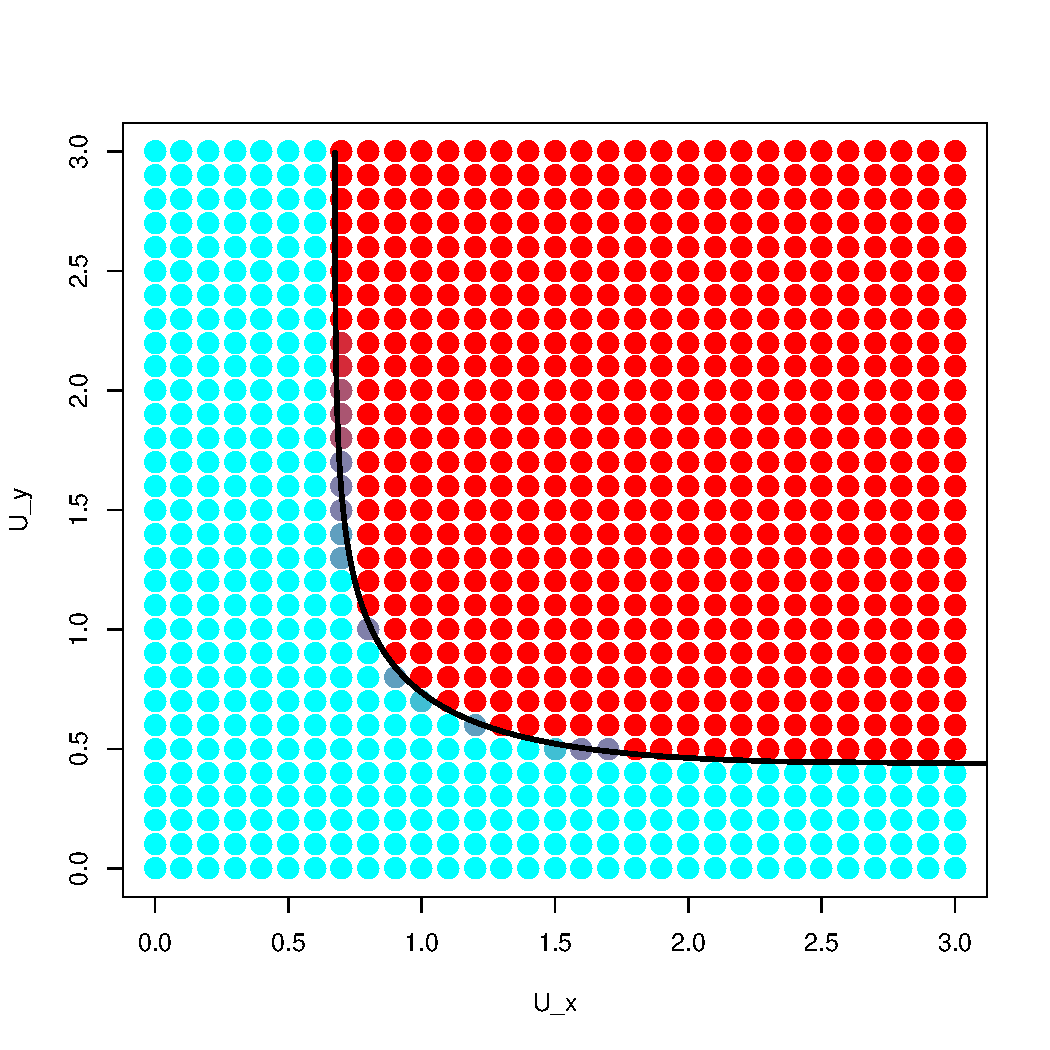
\includegraphics[width=3in]{demo/overlap/color_plot.pdf}
\caption{Number of times $k=2$ is selected out of $10$ replicates for each pair of $(\muX, \muY)$. The heat map shows the frequency $k=2$ is selected by the algorithm, with light means low number (of $k=2$) is selected and dark color means high number is selected. The black line is the theoretical curve, above which the algorithm suppose to pick $k=2$ and below which algorithm select $k=1$.  }
\label{fig:overlap-color_plot}
\end{figure}

\subsection{Correlation adjustment for Gabriel method}
When the correlation between dimensions are high, the proposed Gabriel CV method tends to overestimate the number $k$. A simply remedy for the high correlation is available if we assume common covariance structure among the $k$ clusters. 
\begin{enumerate}
	\item Apply Gabriel CV method on the original data $\dataX$, get estimated number of cluster $\hat{k}$
	\item Estimate the pooled covariance matrix $\hat{\Sigma}$ from the $\hat{k}$ clusters.
	\item Let $\hat{\Sigma} = \Gamma\Lambda\Gamma'$ be the Eigendecomposition of $\hat{\Sigma}$, we rescale and rotate the original data $\dataX$ to get $ \widetilde{\dataX} = \dataX\Gamma\Lambda^{-1/2}Q$, where $Q$ is a random  orthonormal rotation matrix. 
	\item Apply Gabriel CV method again on the transformed data $ \widetilde{\dataX}$ to estimate $k$. 
\end{enumerate}
 

\section{Simulation}
In this section, simulation is performed to evaluate the performance of our
proposed methods in locating the ``correct" number of clusters. We compare
with a basket of existing methods including Gap statistics
\citep{tibshirani2001estimating}, Gaussian mixture model-based clustering
\citep{fraley2002model}, CH-index \citep{calinski1974dendrite}, Hartigan
statistics \citep{hartigan1975clustering}, Jump method
\citep{sugar2003finding}, Prediction strength \citep{tibshirani2005cluster},
Bootstrap stability \citep{fang2012selection} in following simulation
settings. All methods are executed with their default parameter settings. 
We select $p=q$ and $5-$fold cross-validation in row
($m=\frac{1}{4}n$) as default parameter setting for our proposed Gabriel
method. Note that set $p=q$ corresponding to $2-$fold cross-validation in
column. Wold method (detailed in Appendix $A$) and correlation-corrected 
Gabriel method (section $4.3$) are also included for comparison. 

Note that in all settings, cluster centers are randomly generated from 
multivariate normal distribution $\mathcal{N}\left(\mathbf{0},\varsigma \mathbf{I}\right)$. 
All clusters are well-separated, i.e. no overlapping. In fact, any simulated 
clusters with minimum distance less than one unit was discarded, so there is
clear definition of true number of clusters. The parameters $\varsigma$ is chosen 
such that about half of the random realization were discarded. The idea is borrowed from
\cite{tibshirani2001estimating}. The proportion of each method successfully picks the correct
$k$ out of $100$ simulation trials is reported, along with its corresponding confident interval
by Wilson's method \citep{wilson1927probable}.

\begin{enumerate}

  \item \textbf{Correlation between dimensions} -- Six clusters in $10$ dimensions. 
  	Each cluster has $100$ or $50$
    multivariate normal observations with common covariance matrix $\Sigma$ 
    which has compound symmetric structure with $1$ in diagonal and $\rho$ 
    off diagonal. $\rho$ takes value in $\{0,0.1,...,0.9\}$.
	
	\begin{figure}[H]
	\centering
	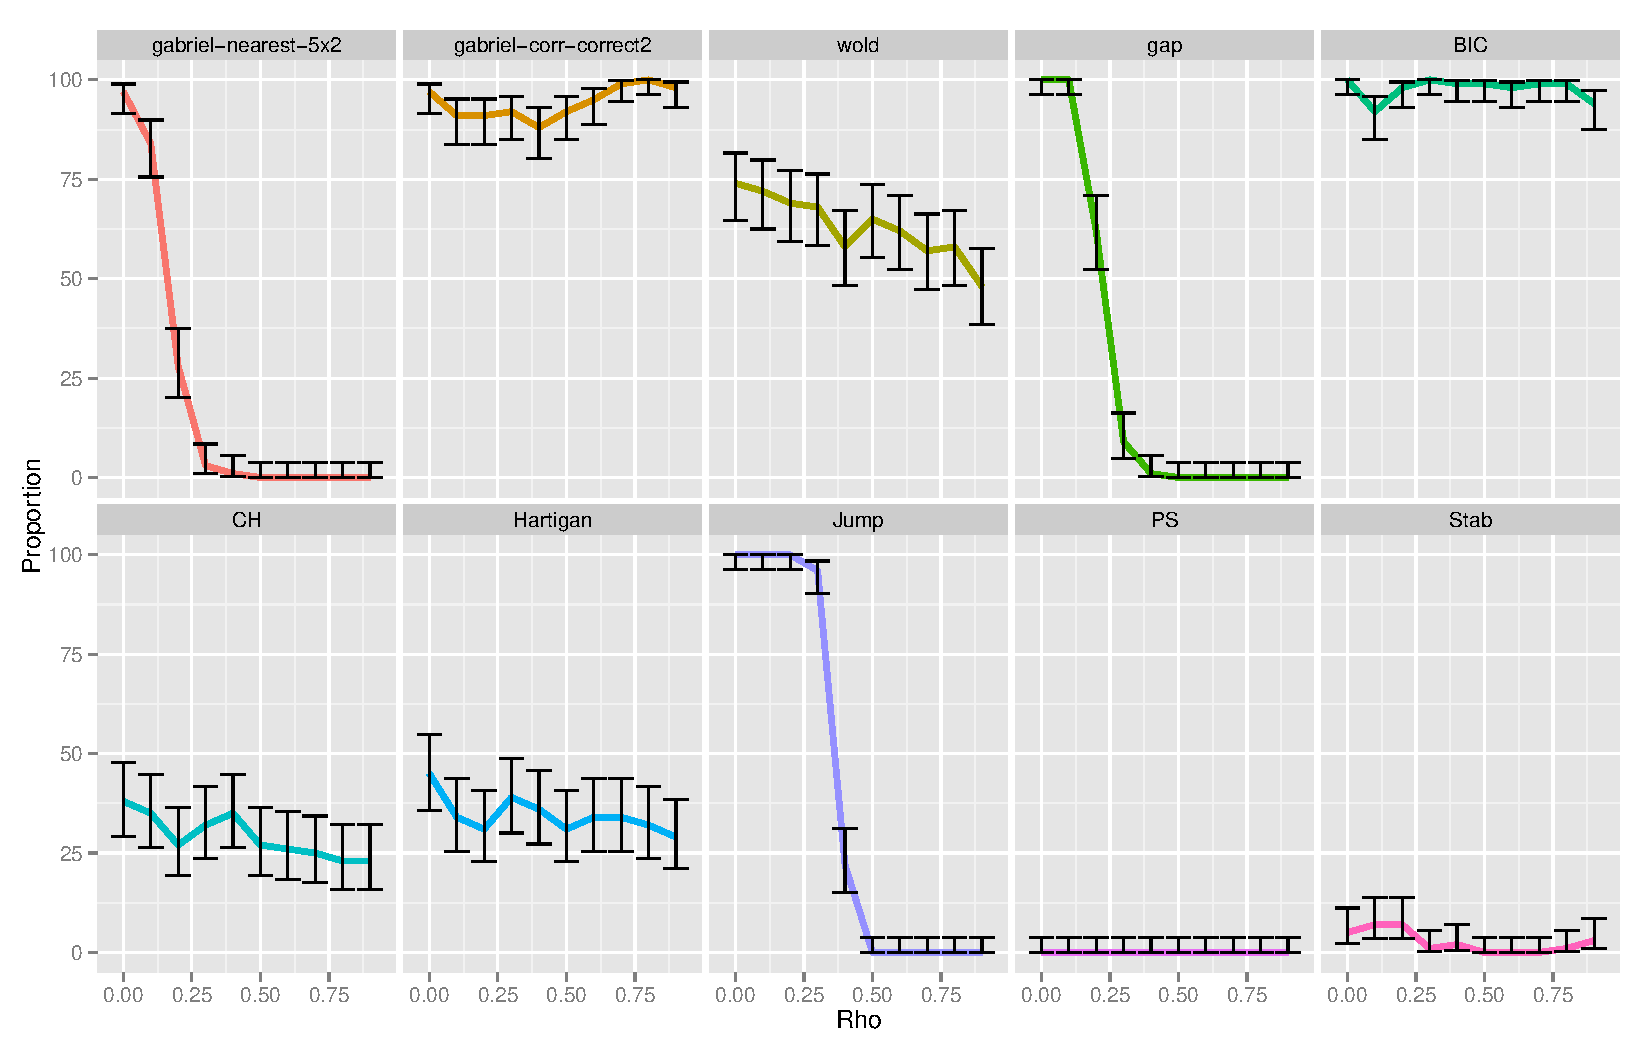
\includegraphics[width=5.5in, height=3.3in]{demo/bench/setting1/Facet.pdf}
	\label{fig:setting1}
	\end{figure}
	
  \item \textbf{Noise dimensions} --- Three clusters in $6$ dimensions. Each cluster has $1000$ or $500$
    mean zero multivariate normal observations with identity covariance matrix. 
    We add $P$ dimensions of noise to the data, which is randomly generated from uniform$[0,1]$. The noise
    dimension $P$ takes values in $\{0,6,...,54\}$. 
	
	\begin{figure}[H]
	\centering
	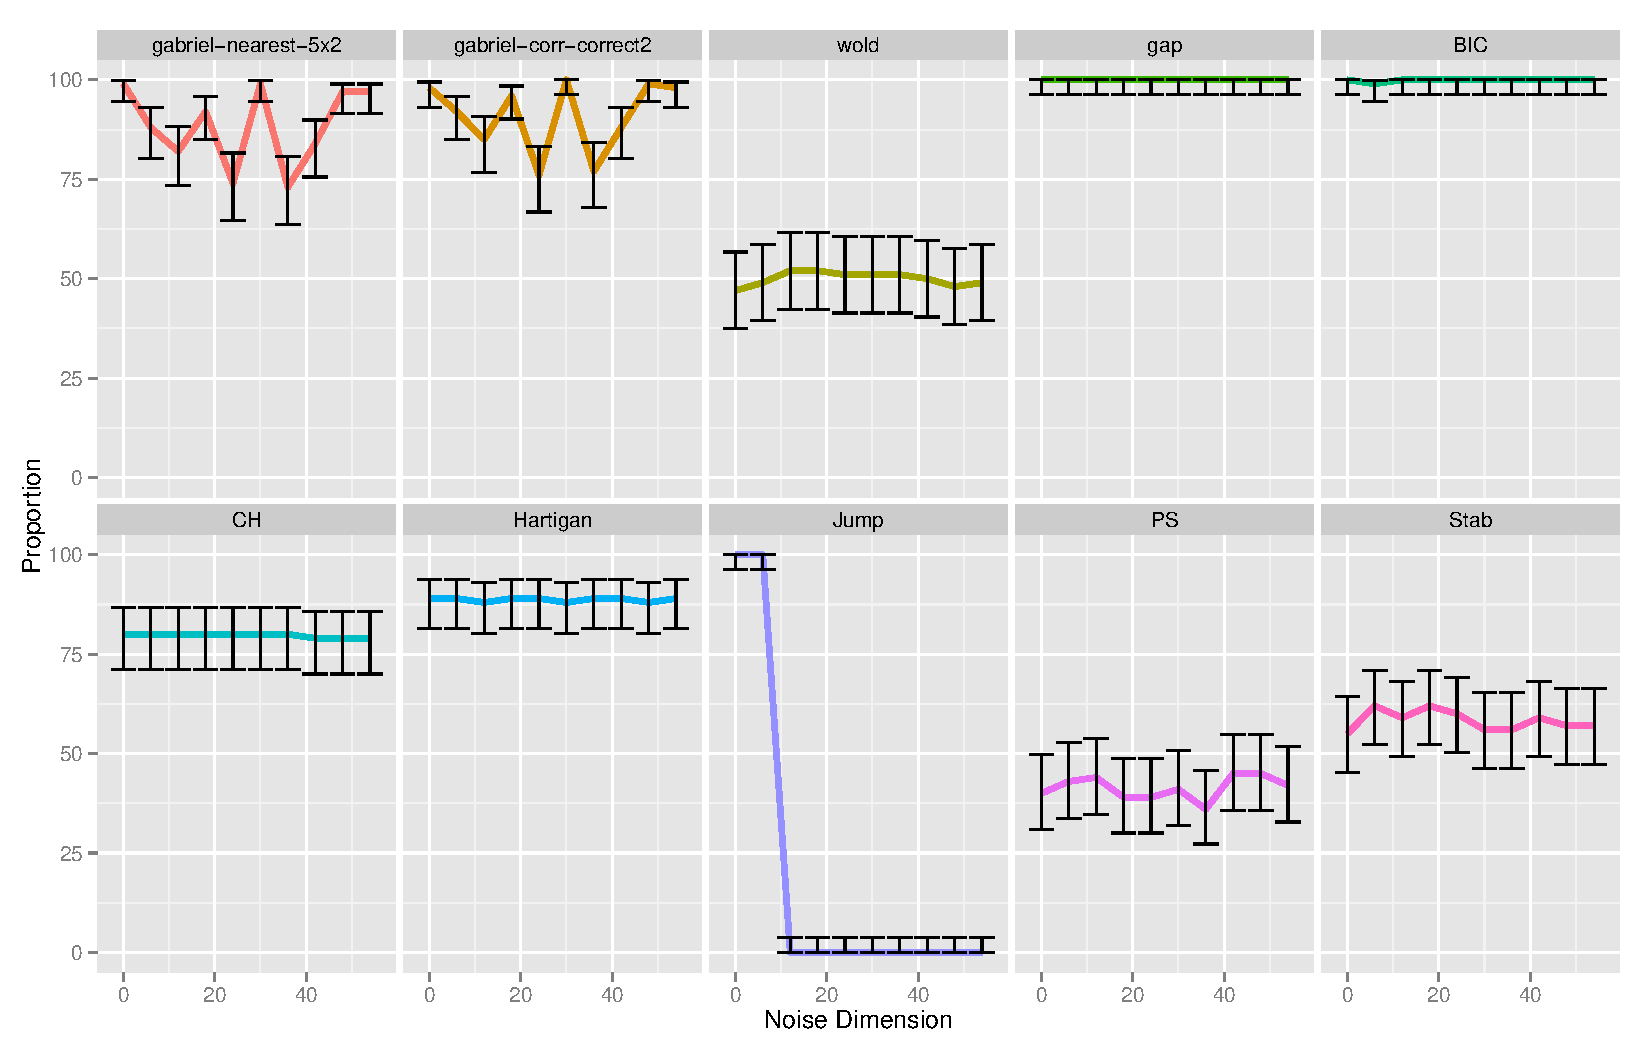
\includegraphics[width=5.5in, height=3.3in]{demo/bench/setting2/Facet.pdf}
	\label{fig:setting2}
	\end{figure}
	
  \item \textbf{High dimension} --- Eight clusters in $p$ dimensions, $p$ takes values 
  	in $\{10,20,...,100\}$. Each cluster has $100$ or $50$ mean zero multivariate normal 
  	observations with identity covariance matrix. 
	
	\begin{figure}[H]
	\centering
	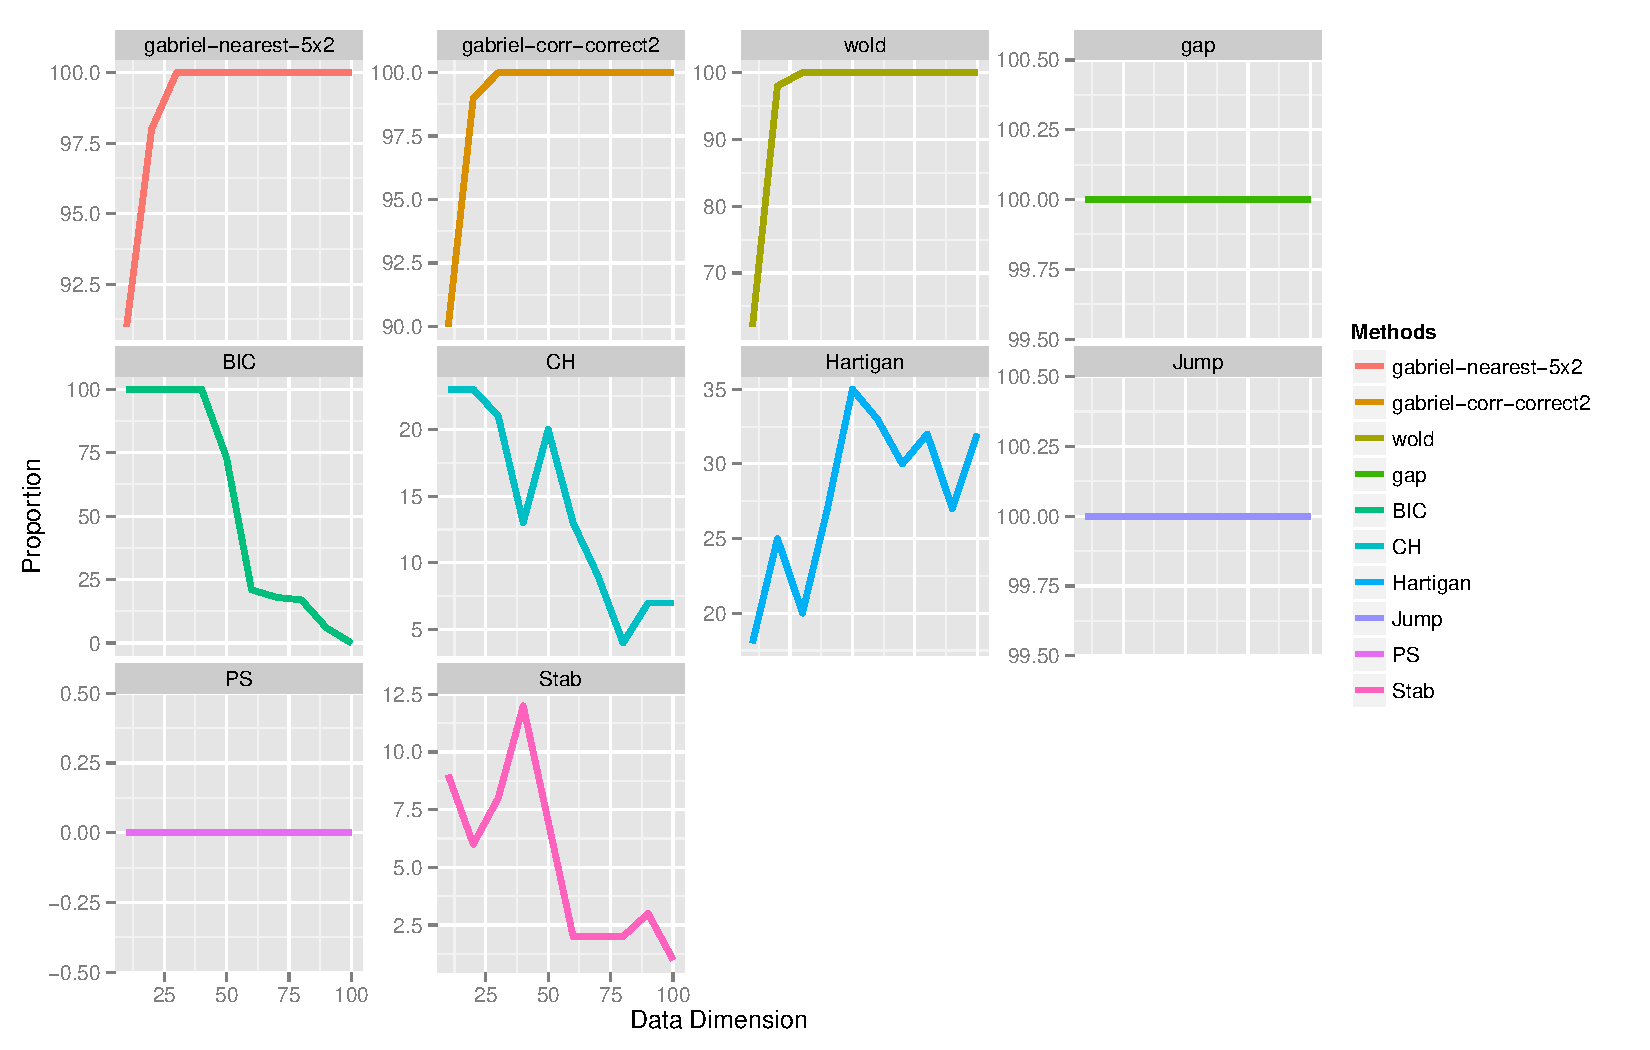
\includegraphics[width=5.5in, height=3.3in]{demo/bench/setting3/Facet.pdf}
	\label{fig:setting3}
	\end{figure}
	
     \item \textbf{Variance heterogeneity} --- Three clusters in $20$ dimensions, each has
     $60$ observations in it. Observations are generated from 
     $\mathcal{N}\left(\mathbf{0},\sigma_1^2\mathbf{I}\right)$,
      $\mathcal{N}\left(\mathbf{0},\sigma_2^2\mathbf{I}\right)$ and
       $\mathcal{N}\left(\mathbf{0},\sigma_3^2\mathbf{I}\right)$ where 
       $\sigma_1^2 : \sigma_2^2: \sigma_3^2 = 1:\frac{1+R}{2}:R$. The maximum ratio $R$
       takes values in $\{1,5,10,...,45\}$
	
	\begin{figure}[H]
	\centering
	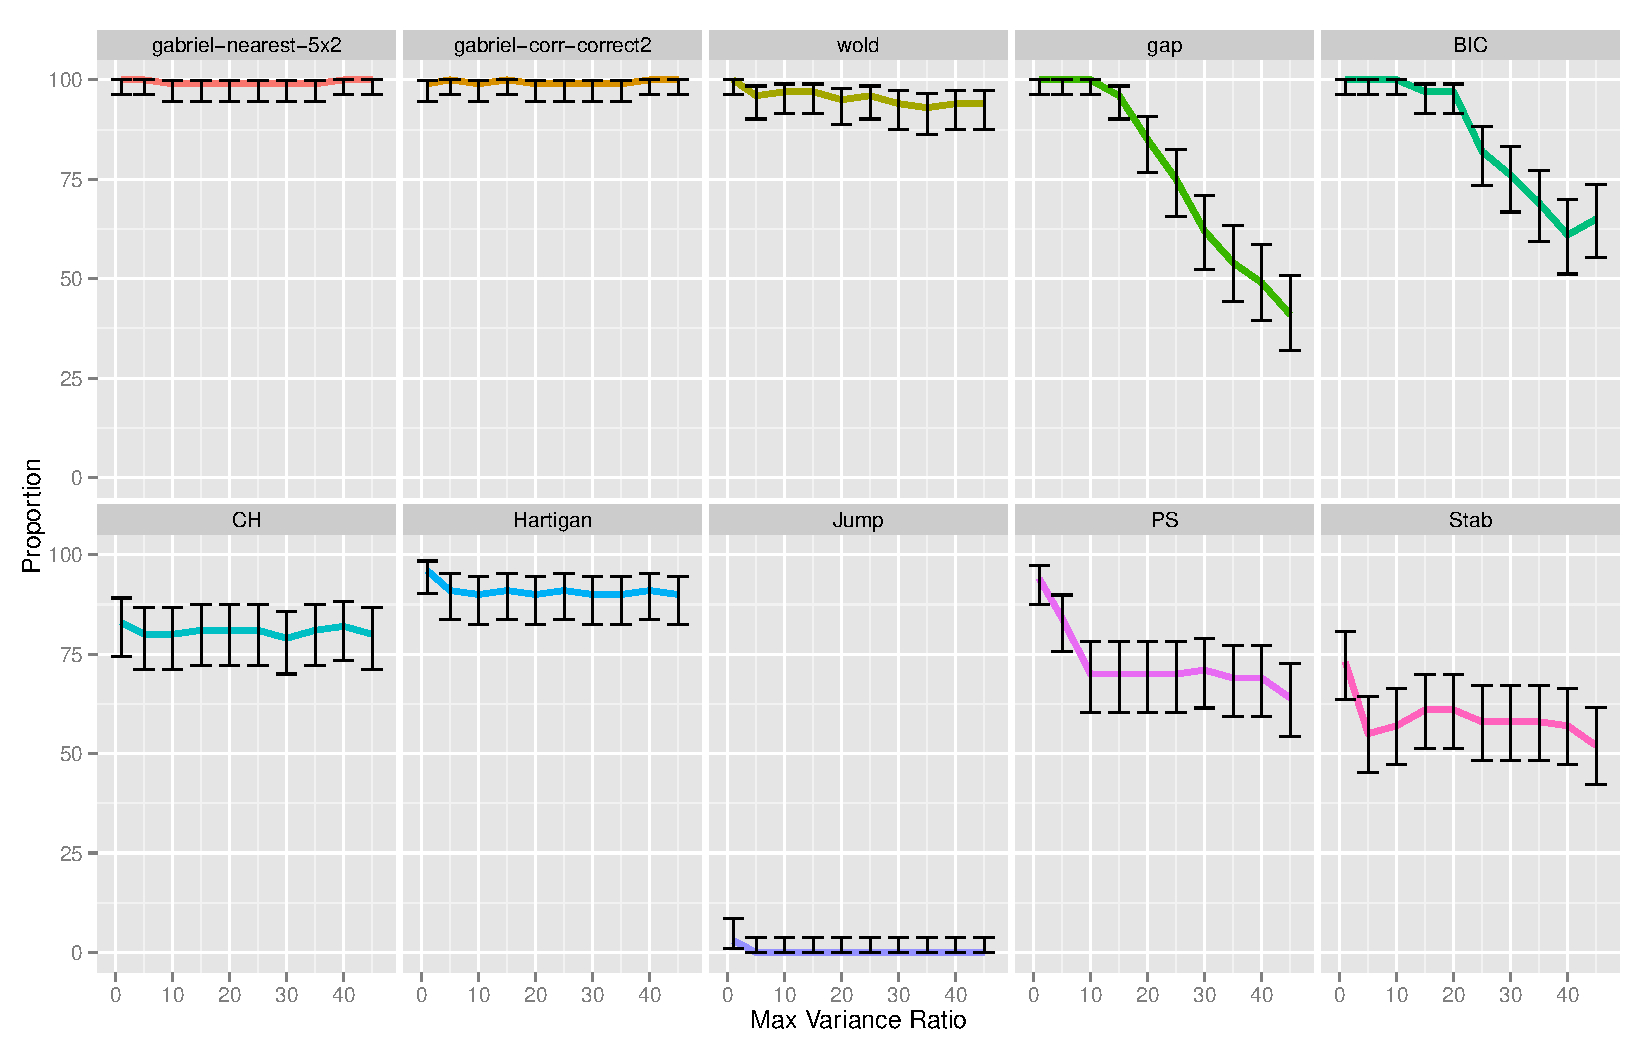
\includegraphics[width=5.5in, height=3.3in]{demo/bench/setting4/Facet.pdf}
	\label{fig:setting4}
	\end{figure}
	
	\item \textbf{Heavy tail data} --- Five clusters in $15$ dimensions, each has
     $80$ observations in it. Observations have independent $t$ distribution in each dimension  
     with degree of freedom $\nu$, which takes value in $\{11,10,...,2\}$
     
	\begin{figure}[H]
	\centering
	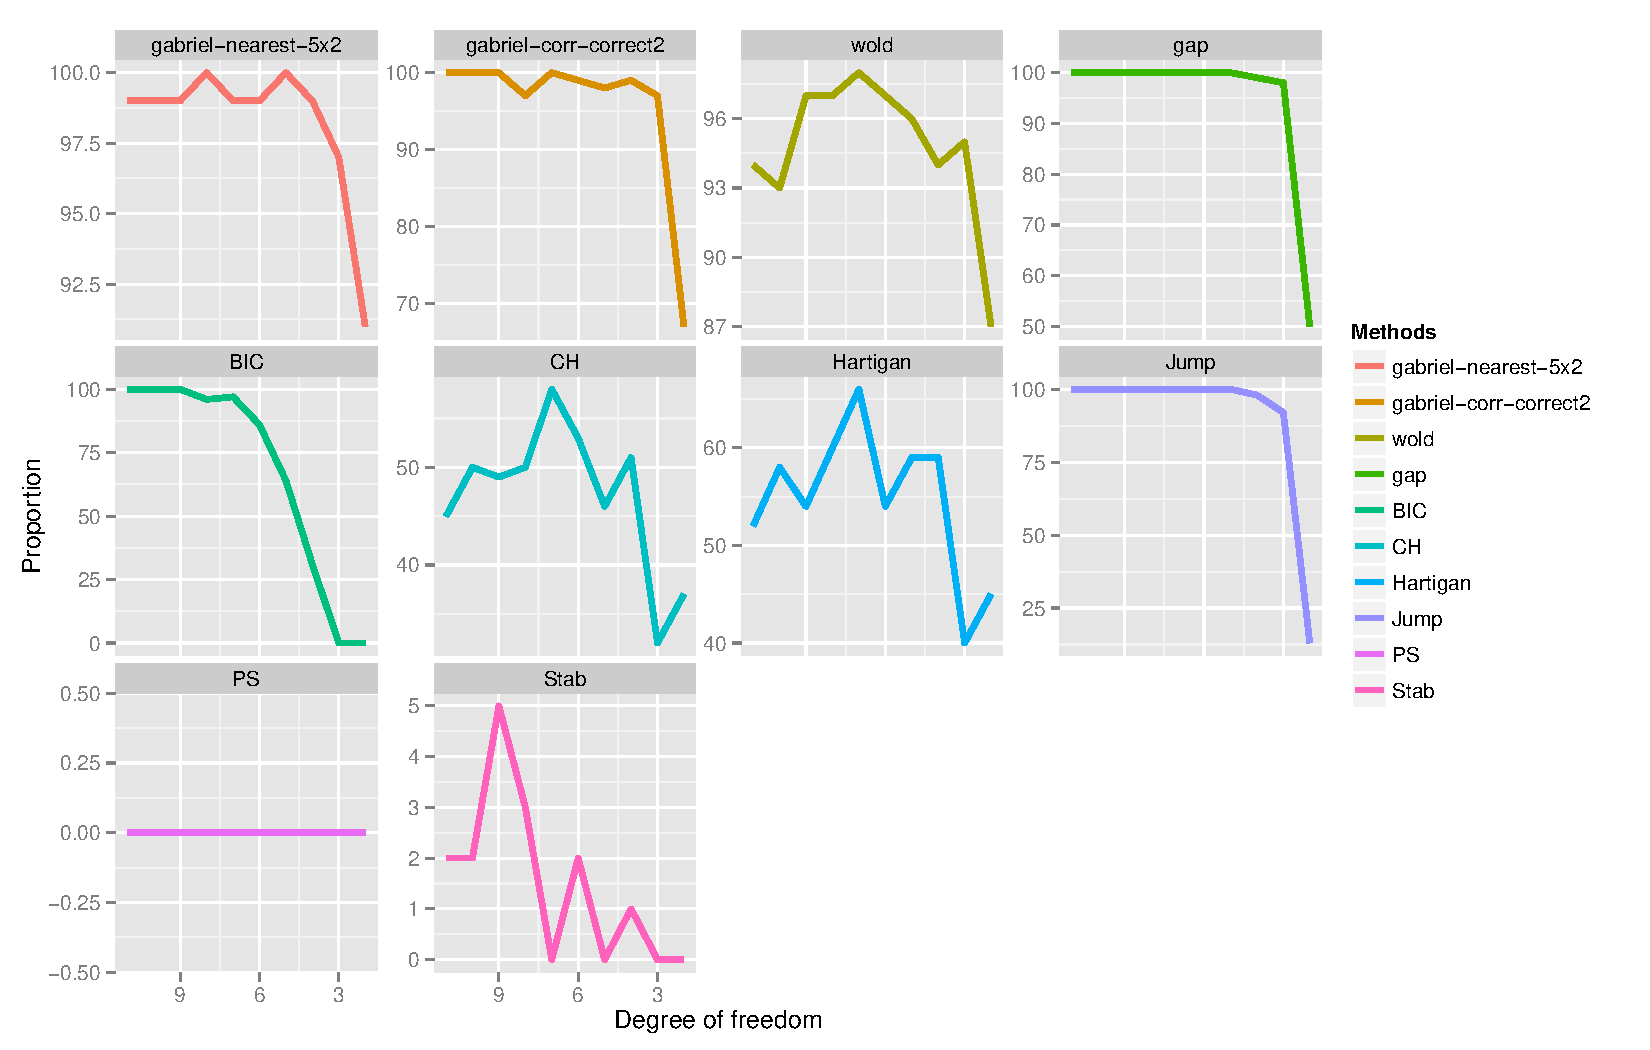
\includegraphics[width=5.5in, height=3.3in]{demo/bench/setting5/Facet.pdf}
	\label{fig:setting4}
	\end{figure}
\end{enumerate}

From the graph of setting $1$, we can see high correlation between dimensions cause problem for most 
existing methods as well as the proposed Gabriel CV method and Wold method. Higher correlation clearly 
degenerate most algorithms' ability to find the correct $k$ as data no longer spherical in $p$-dimension.
And the recent proposed methods (Gabriel CV method, Gap statistic, Jump method) seem to be more sensitive to
high correlation than those old methods such as CH-index and Hartigan statistics. The only two methods 
work well in high correlation are the Gaussian model-based BIC method \citep{fraley2002model} and the 
correlation-corrected Gabriel method. 

Plot of setting $3$ shows some methods are insensitive to higher dimension such as Jump method and Gap 
statistics, while others deteriorate quickly with increasing dimension, most notably the Gaussian 
model-based BIC method. Note here the data are still generated from mixture of Gaussian. In contrast, our 
proposed Gabriel CV method as well as its correlation-corrected version actually working better in higher 
dimension. 

Result of setting $4$ indicates most previously methods are sensitive to variance heterogeneity among 
clusters, most notably the Gap statistics and model-based BIC method. The proposed Gabriel CV method
and its correlation-corrected version consistently perform well in estimating $k$ and quite insensitive
to variance heterogeneity. The Wold method also performs well in this setting.   

The last non-Gaussian setting examines methods' performance in heavy-tail data. With degree of freedom 
decreases, the tail becomes more flat and the Gaussian assumption becomes more inappropriate. It explains
the sharp plunge of Gaussian model-based BIC method in the plot. For most methods, their performances are 
relatively stable until the tail gets very heavy. In case where degree of freedom is $2$, Gap statistics 
and Jump method dived considerably compare to the Gabriel method and Wold method. 

In conclusion, the proposed Gabriel CV method compares well with current state-of-the-art methods and 
is very robust against variance heterogeneity, high dimension and heavy-tail data. One weakness of the 
Gabriel CV method is that it's sensitive to the high correlation among dimensions. In such case, its 
correlation-corrected version will perform well under the assumption of common covariance structure. 

\section{Real data application}
We also applied our proposed method to three real world data sets, two were obtained
from the University of California Irvine machine learning repository. The
first and third data sets are selected because there are clear number of
clusters in those two data sets. The second data set is used as a benchmark
data set since it was widely used in literature.

The first one is congress voting data which consists of voting records of
$98$th United States Congress, $2$nd session \citep{schlimmer1987concept}. 
This data set includes votes for each of the U.S. House of Representatives Congressmen on the $16$ key votes
identified by the \textit{CQA} (Congressional Quarterly Almanac). For each
vote, each Congressman either vote positively ``yea" (voted for/paired
for/announced for),  negatively ``nay'' (voted against/paired
against/announced against) or position unknown ``?". We took out those records
contain ``?" before comparing each algorithm. It results in $232$ remaining
records, with $124$ democrat and $108$ republican. 

The second data set is the well-known Wisconsin breast cancer data set \citep{mangasarian1990pattern}. After excluding the records with missing data, this data set consists records of $683$ patients, each with measurements of nine attributes of their biopsy specimens. It is known that there exist at least two groups of patients: $444$ patients with benign specimens and $239$ patients with malignant specimens.


The third data set is gene expression data of $5$ types of brain tumours from \cite{de2008clustering}, which contains $42$ observations including $10$ medulloblastomas, $10$ malignant gliomas, $10$ atypical teratoid/rhabdoid tumours (AT/RTs), $8$ primitive neuroectodermal tumours (PNETs) and $4$ normal cerebella. It was originally used by \cite{pomeroy2002prediction} to show that medulloblastomas are molecularly distinct from other types of brain tumours.

Data was collected with Affymetrix microarrays, which estimates the number of RNA copies found in the cell sample (frozen specimens). Data was preprocessed as following: as a common procedure, all genes with expression level below $10$ are set to a minimum level threshold of $10$. The maximum threshold is set at $16,000$. Values below or above these thresholds are often unreliable. To remove uninformative genes, for each gene $j$ (attribute), the mean $m_j$ among the samples was calculated. The $10\%$ largest and smallest values are discarded in order to remove extreme values. Based on the mean, following transformation is applied on every value $x_{ij}$ of sample $i$ and gene j
\[	y_{ij} = \log_2 (x_{ij}/m_j)	\] 
Genes with expression levels differing by at least $l$-flod in at least $c$ samples from their mean expression level across the sample were selected. The parameter $l$ and $c$ were chosen so as to produce a filtered data set with at least $10\%$ of the original number of genes \citep{de2008clustering}. Such preprocessing procedure results in $1379$ genes selected. After filtering step, data is restored in the original scale (i.e. $x_{ij}$). So the data set is $42 \times 1379$, which serves as a high dimensional example.


\begin{table}[H]
\begin{center}
\captionsetup{justification=centering}
\caption{\label{table2} Number of clusters selected by each algorithm}
\begin{tabular}{lccccc}
    \hline                  
 & Congress Voting && Breast Cancer && Brain Tumours \\ \hline                    
CH-index & $2$ && $2$  && $2$    \\
Hartigan & $3$ && $3$  &&  $4$   \\
Jump & $10$ && $9$ && $1$  \\   
Prediction strength & $2$ &&  $2$ && $1$    \\
Bootstrap stability & $2$ &&  $2$ &&  $7$   \\ 
Gap & $8$ && $10$ && $10$  \\   
Gaussian-BIC & $2$ && $5$ && $2$  \\   
Gabriel & $2$  && $3$  && $5$  \\    
Gabriel-corr-correct & $2$  && $2$  && $5$  \\  
Wold & $2$ && $3$ && $4$ \\  \hline 

\end{tabular}
\end{center}
\hspace{0.5in} \footnotesize {All the algorithms executed with their default parameter settings with $k$ ranges from $1$ to $10$}
\end{table} 

Since most congressmen vote based on their parties' interest, two parties
(Democratic and Republican) represent two clusters in this data set. So the
optimal number should be two. Close inspection shows $k$-means with
$k=2$ separates the two parties very well with the lowest miss-classification
error $10.43\%$ ($k=3$ has $14.78\%$). Our proposed Gabriel CV method, along with 
several other algorithms correctly pick $k=2$ for this data set. Note that CH-index and Bootstrap
stability also return $k=2$, but $2$ is the lower bound those methods can
select for $k$. So it's not clear they actually choose $k=2$ or they hit the
lower bound (they would pick $k=1$ if allowed). 

For the breast cancer data, it's known to have $2$ clusters based on 
whether it's benign specimens or malignant specimens. Although the proposed Gabriel method
picks $k=3$, its correlation-corrected version correctly picks $k=2$. It shows the necessity 
to correct for the high correlation among data features. However, for this data $k=3$ is also
an acceptable answer, as \cite{fujita2014non} noticed that the malign group is quite heterogeneous and
can be further clustered into at least two subgroups.

The brain tumours gene expression data is a typical high-dimension data with $p > n$. It is clear that 
the correct number of clusters should be $5$, the number of brain tumour types. Indeed, $k$-means results with $k=5$ show that the $4$ normal human cerebella are well separated from brain tumours as they form a single cluster.  
Medulloblastomas, malignant gliomas and AT/RT tumours also form $3$ respective clusters, which means they can be separated from each other. Such results are similar to those found in \cite{pomeroy2002prediction}, whose analysis
is based on the first $3$ principle components of the original data.    
From table \ref{table2} we can see only our proposed Gabriel method (as well as its correlation-corrected version) correctly selects $k=5$, underline how difficult it was to pick the right $k$ when dimension is high. 


\subsection{Application on Yeast data set}
The yeast Saccharomyces cerevisiae data set was collected by \cite{cho1998genome} to study the genome-wide characterization of mRNA transcript levels during the cell cycles of the budding yeast S. cerevisiae. To obtain data, 
cdc28-13 cells were synchronized in late G1 phase by heat treatment, and the cell cycle was reinitiated by shifting cells to cooler temperature. Data was collected at $17$ time points at every $10$ minutes intervals covering almost $2$ complete cell cycles. Oligonucleotide microarrays was used to query $6,220$ gene expression profiles at these $17$ time points. This data has been the subject of several studies and is generally accepted as a reference \citep{dortet2008model}.    

\cite{tavazoie1999systematic} applied $k$-means clustering on the preprocessed data with $k=30$ and discovered several periodic clusters. The preprocessing procedure includes choosing the most variable $2,945$ geness among the total $6,220$ by metric of variation based on the normalized dispersion across time points (s.d/mean). Data at time points $90$ and $100$ minutes were removed because of their less efficient labelling of mRNA during the original chip hybridization. It results a $2,945$ by $15$ data matrix. The last step of the preprocessing procedure is to variance normalize each gene across the $15$ time points, which is done by subtracting the mean and then dividing by the standard deviation. The result is each gene has mean zero and standard deviation equal to one across the time points.

\cite{dortet2008model} performed model-based clustering on the preprocessed data of \cite{tavazoie1999systematic} and  found $27$ clusters. They classified the $27$ clusters into $3$ major types: cyclic gene clusters, stress gene clusters and the clusters neither cyclically nor sensitive to the induced stress. 

We also applied our proposed Gabriel method on the preprocessed data of \cite{tavazoie1999systematic}. The algorithm found $5$ clusters. Since the dimensions (time points) are likely to be correlated, we also applied the correlation-corrected version of Gabriel method on the data which also result $5$ clusters. This numbers is much smaller compare to those of \cite{tavazoie1999systematic} and \cite{dortet2008model}. We will focus our analysis on this $5$ clusters found by the proposed method, whose result is summarized on the top panel of Figure \ref{fig:5_clusters}, where each cluster is presented by the mean expression level of all the genes within that cluster over $15$ time points. Similar as \cite{tavazoie1999systematic}, we found the members of each cluster to be significantly enriched for genes function in similar biological process. Each gene is mapped with the Gene Ontology (GO) Annotation in Saccharomyces Genome Database (SGD) database, which provides Gene Ontology (GO) annotation of the entire genome using GO slims, which are high-level subsets of GO terms that allow grouping of genes into broad categories, such as biological process, molecular function or cellular component. We choose to group genes in terms of biological process, which is a recognized series of events or molecular functions. There are total $103$ categories for biological process.

To identify biologically meaningful gene clusters from spurious ones, \cite{tavazoie1999systematic} introduced a method, enrichment analysis, to assess the statistical significance of the over-represented gene class in a cluster using hypergeometric distribution. Specifically, the $p$-value of observing $k$ genes from a particular category group within a cluster of size $m$ is given by:
\[	P = 1-\sum^{k-1}_{i=1} \frac{{{2945-n}\choose{m-i}}{{n}\choose{i}} }{ {{2945} \choose{m}} }\] 
where $n$ is the total genes in that group. It can be seen as testing the null hypothesis that genes are randomly  distributed among each cluster. The categories with the most significant grouping of gene inside each of the $5$ clusters are shown in Table \ref{table:enrich}.

To better compare our results with those of \cite{tavazoie1999systematic}, we also prepared confusion Table \ref{table:confusion} and Figure \ref{fig:5_clusters}. The number in cell $(i,j)$ of Table \ref{table:confusion} shows the number of observations that belong to both the $i$th cluster of ours and the $j$th cluster of \cite{tavazoie1999systematic}. The plots in Figure \ref{fig:5_clusters} have similar meaning -- the mini plot on first row and the $4$th column is the mean gene expression level of observations belong to both the first cluster of \cite{tavazoie1999systematic} and the $4$th cluster of ours. We only plot the mean expression level if the number of observations in that cell is greater than $20$. Although \cite{tavazoie1999systematic} found $30$ clusters, not all of them were discussed in \cite{tavazoie1999systematic}. We only compare our results with those clusters that were profiled in \cite{tavazoie1999systematic}. The complete confusion matrix is in Appendix \ref{app:confusion}. The original result of \cite{tavazoie1999systematic} is obtained from site \url{http://arep.med.harvard.edu/network_discovery/}.


\begin{table}
\begin{center}
\captionsetup{justification=centering}
\caption{\label{table:enrich} Enrichment of clusters for genes within biological process categories}
\scalebox{0.8}{%
\begin{tabular}{cclcl}
\hline
   Cluster & Cluster size($m$) & Biological process category(total genes) & genes within category($k$) &$p$-value \\ \hline
 $1$ & $550$  &  response to oxidative stress ($55$)  &    $24$  & $1.5\times10^{-5}$ \\
     &     &  response to chemical ($213$)    &    $64$     & $2.2\times10^{-5}$\\
  $2$& $590$  &  mitochondrion organization ($159$) & $79$ &  $1.1\times10^{-16}$  \\  
  	 &     &  mitochondrial translation ($51$) & $28$ 	&  $2.9\times10^{-8}$  \\  
  	 &     &  generation of precursor metabolites and energy ($80$) &  $37$ & $7.3\times10^{-8}$   \\  
 $3$ & $654$ &  transcription from RNA polymerase II promoter ($214$) & $75$ &  $5.5\times10^{-6}$    \\  
  	 &     & mRNA processing ($67$) & $30$ 	& $2.7\times10^{-5}$    \\  
  	 &     & mitotic cell cycle ($183$)  & $63$ 	& $6.2\times10^{-5}$  \\ 
  $4$& $634$  & cytoplasmic translation ($134$)  &  $105$ &  $3.3\times10^{-47}$   \\  
     &     &  ribosomal subunit biogenesis $(138)$ & $73$ 	&  $7.7\times10^{-17}$  \\  
  	 &     &  rRNA processing ($131$) &  $61$	&  $5.7\times10^{-11}$  \\  
  	 &     &  ribosome assembly ($36$) &  $21$	&  $1.5\times10^{-6}$  \\  
$5$  &   $517$   &  chromosome segregation($106$) &  $53$      &  $6.0\times10^{-15}$ \\
     &     &  cellular response to DNA damage stimulus ($172$)  &  $71$  & $3.6\times10^{-14}$     \\  
  	 &     &  DNA repair ($147$)  &  $64$  & $3.7\times10^{-14}$     \\                 
 	 &     &  DNA replication ($78$)  & $42$   &  $1.8\times10^{-13}$   \\  
  	 &     &  mitotic cell cycle ($183$)  &  $70$  &  $4.8\times10^{-12}$   \\  
 


\hline
\end{tabular}
}
\end{center}
\hspace{0.5in} \footnotesize {}
\end{table} 

It turns out that each cluster has unique trend of expression level and contains genes that tend to participate in the common processes. Cluster $1$ has decreasing expression level with time. From Table \ref{table:enrich}, we can see it concentrates genes that somatize the cell stress, such as oxidative heat-induce proteins. It mainly consists of observations that did not get profiled in \cite{tavazoie1999systematic}, as we can see from Table \ref{table:confusion} and Figure \ref{fig:5_clusters}.

The mean gene expression level in Cluster $2$ decreases at the beginning and then increase. Our analysis found genes govern mitochondrial translation and mitochondrion organization are heavily concentrated in cluster $2$. Genes in \cite{tavazoie1999systematic}'s cluster $4$ and $8$ are heavily concentrated in this cluster, which also explains the coincidence between the enriched categories in our cluster $2$ and the functional groups in cluster $4$ and $8$ of    \cite{tavazoie1999systematic}.

Our cluster $3$ is a periodic cluster where one can see two gene expression cycles from Figure \ref{fig:5_clusters}. Indeed, cell cycle genes that related to budding and cell polarity are commonly found in cluster $3$. In addition, one can see from Table \ref{table:enrich} that genes govern RNA processing and transcription are highly represented in this cluster. Comparing cluster $3$ to the clusters found in \cite{tavazoie1999systematic} from Table \ref{table:confusion} and Figure \ref{fig:5_clusters}, one can see that it mainly consists of genes from cluster $3$, $7$ and $14$ of \cite{tavazoie1999systematic}. Note that the cluster $7$ and $14$ are both periodic clusters highlighted in \cite{tavazoie1999systematic}.

Cluster $4$ has increasing expression level with time. From Table \ref{table:enrich}, we can see genes related to cytoplasmic translation are highlighted in this cluster. Genes encode ribosomes are also overly presented in cluster $4$. This cluster corresponding to cluster $1$, the most notable functional grouping cluster of \cite{tavazoie1999systematic}. Indeed, one can see from Table \ref{table:confusion} that almost entire cluster $1$ of  \cite{tavazoie1999systematic} is contained in our cluster $4$.

One can easily see from Figure \ref{fig:5_clusters} that our cluster $5$ is also a periodic cluster. Enrichment analysis shows that genes participated in the cell-cycle phase related processes such as DNA replication and DNA repair are highly concentrated in this cluster. Table \ref{table:confusion} shows that the entire cluster $2$ of \cite{tavazoie1999systematic} is contained in our cluster $5$, along with some genes from cluster $14$. Note that both cluster $2$ and $14$ are profiled periodic clusters in \cite{tavazoie1999systematic}. We can also see from Figure \ref{fig:5_clusters} that our cluster $5$ groups together genes with similar cycle phase in \cite{tavazoie1999systematic}'s cluster $2$ and $14$. 

In conclusion, our clusters group together genes that participate in the common biological processes. Our results are broadly align with the results in \cite{tavazoie1999systematic}, which clustered the data with $k=30$. In particular, the periodic cell cycle related genes are concentrated in cluster $5$ and cluster $3$, which consistent with the findings in \cite{tavazoie1999systematic} (cluster $2$, $7$ and $14$). Indeed, more than $70\%$ genes which function in mitotic cell cycle process are concentrated in these two clusters. The number of clusters found by our method is much smaller than the number of clusters used in \cite{tavazoie1999systematic} and \cite{dortet2008model}. However, both studies found that most of their clusters have no characteristics, suggesting overestimate of the underlying diversity of biological expression classes in the data set \citep{tavazoie1999systematic}. From Figure \ref{fig:5_clusters}, one can see clusters in \cite{tavazoie1999systematic} with similar behavior are merged in our cluster, which leads to smaller number of clusters. Our result is more parsimonious, while still able to identify the functional grouping of genes in clusters highlighted in previous studies.


	\begin{figure}[H]
		\centering
	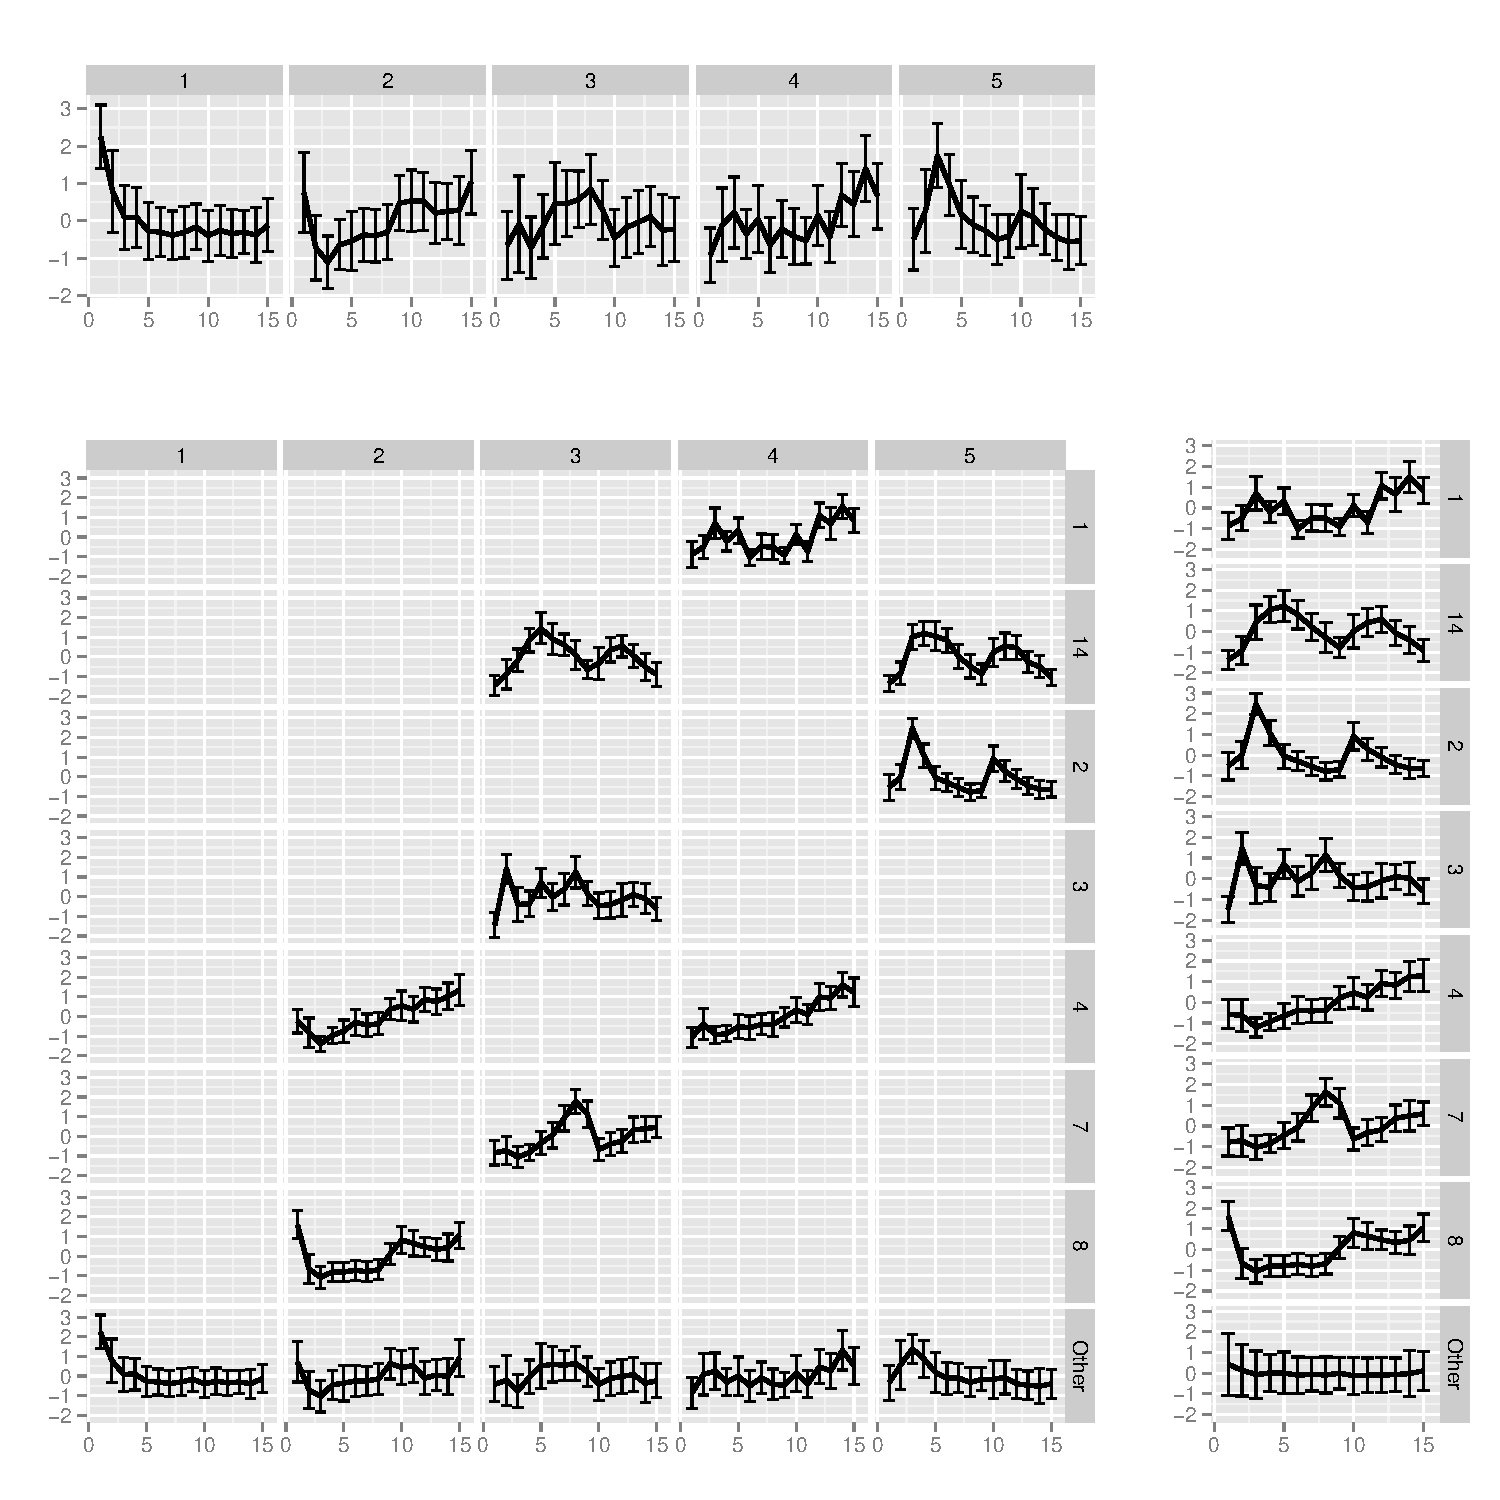
\includegraphics[width=6.2in, height=6.2in]{wei/split_plots.pdf}
	\caption{Yeast data set mean expression profiles. The $5$ clusters found by Gabriel method are on the top; Clusters profiled in \cite{tavazoie1999systematic} are on the right.}
	\label{fig:5_clusters}
	\end{figure}

\begin{table}[t]
\begin{center}
\captionsetup{justification=centering}
\caption{\label{table:confusion} Confusion matrix comparing $5$ clusters to $30$ clusters }
\begin{threeparttable}
\begin{tabular}{lccccccc}
\hline
   &  Cluster $1$  & Cluster $2$   &  Cluster $3$  &  Cluster $4$ &  Cluster $7$  & Cluster $8$  & Cluster $14$ \\ \hline 
 Cluster $1$  & $0$  &  $1$  & $0$  &  $0$  & $1$  & $3$  & $0$ \\
 Cluster $2$  & $0$  &  $0$  & $0$  & $102$ & $10$ & $145$& $1$ \\
 Cluster $3$  & $1$  &  $0$  & $91$ &  $2$  & $83$ & $0$  & $29$ \\
 Cluster $4$  & $161$&  $0$  & $11$ &  $66$ & $7$  & $0$  & $6$ \\
 Cluster $5$  & $2$  & $185$ & $2$  &  $0$  & $0$  & $0$  & $38$ \\ \hline      
\end{tabular}
 \begin{tablenotes}[para,flushleft]
\footnotesize {Only the profiled clusters in \cite{tavazoie1999systematic} are listed here}.
  \end{tablenotes}
\end{threeparttable}
\end{center}
\end{table} 	

\section{Discussion}
\label{sec:conc}
In this paper, we proposed a novel approach to estimate the number of
clusters. The intuition behind our proposed methods is to transfer the
unsupervised learning problem into supervised learning problem via novel form
of cross validation. Such approach is quite different from previous methods which 
utilize the within/between cluster dispersion or stability criterion for selecting the 
optimal $k$. Our method utilizes the connection between different dimensions (columns)
of data through the uniqueness of each cluster center. We proved the self-consistency 
for our proposed Gabriel CV method as well as its asymptotic property with Gaussian noise,
and showed the robustness of our method by simulation. Our method has very good performance
in our limited simulation settings and real data application, and clearly the superior
one when data has heterogeneous variance or is heavy-tailed.

Besides no strong modeling assumption is required, our proposed method is robust against data set 
with variance heterogeneity, unequal number of observations, non-Gaussian noise and high-dimension. 
Such robustness is important in practice because for any given data, it's hard to tell whether
its clusters have different number of observations, is the variance equal for each cluster,
or what underlying noise distribution it has. The weakness of our proposed method is 
that its theory assumes only week correlation between ``predictor'' columns and ``response'' 
columns. In practice, many data sets don't exhibit high correlations between columns, where
our proposed method can be safely applied. In case the high correlation does exist, 
the correlation-corrected version of Gabriel CV method in section $4.3$ can be used if we can 
assume common covariance structure. Other procedure such as leave out most columns for clustering 
may also be used to reduce its effect. However, the theory for such procedure has not
been fully developed and it could be the future research topic. 

Another situation where our proposed method cannot be directly used is when the clusters 
are non-convex. In such situation, $k$-means itself doesn't work well, for example two 
concentric circles share the same cluster center \citep{hastie2009elements}. However, it's 
possible that our proposed Gabriel CV method can be used on the transformed data set. In the
concentric circles case where spectral clustering is appropriate, our proposed method can be applied 
on the eigenvector subspace of the graph Laplacian matrix inside the spectral clustering algorithm
to find the optimal $k$. This can also be the future research topic. 

\clearpage

\section*{\textbf{APPENDIX}}
\appendix
\section{Wold CV estimation} \label{app:foobar}
\begin{itemize}
	\item For each $k = 1,2,...,k_{max}$
	\begin{enumerate}
		\item Randomly draw some entries in $\mathbf{X}$ missing, keep those hold-out values in vector $V_{true}$
		\item Impute the missing values with column mean or $0$, denote the imputed data as $\mathbf{X}_{new}$
		\item Apply the iterative procedure below until converge or stopping criteria reached
		\begin{itemize}
			\item Apply $K$-mean on data set $\mathbf{X}_{new}$ with parameter $k$
			\item Substitute each observation in $\mathbf{X}_{new}$ by its nearest center, get new data $\mathbf{X}^c_{new}$ ($\mathbf{X}_{new}$ keep the same)
			\item Replace (impute) those imputed values in $\mathbf{X}_{new}$ with the corresponding entries in $\mathbf{X}^c_{new}$
			\item Calculate the difference between the old and newly imputed values, check whether or not they coincide (converge) 
		\end{itemize}
		\item Obtain the last imputed entry values of converged $\mathbf{X}_{new}$, denote it by $V_{converge}$
		\item Calculate the prediction error  $Error_k = ||V_{true} - V_{converge}||^2$ 
	\end{enumerate}
	\item For each CV folder, repeat above procedure and obtain the $Error_k$ for each $k$
	\item Average $Error_k$ across all folders for each $k$, and then select the $k$ corresponding to the minimum average $Error_k$ 
\end{itemize}

\section{Technical Lemmas}
\label{app:technical-lemmas}

\begin{lemma}\label{lem:truncated-normal-moments}

If $Z$ is a standard normal random variable, then
\[
  \E(Z \mid a < Z < b)
    = - \frac{\varphi(b) - \varphi(a)}
             {\Phi(b) - \Phi(a)}
\]
and
\[
  \E\{(Z - \delta)^2 \mid a < Z < b\}
    = \delta^2 + 1
    - \frac{  (b - 2 \delta) \varphi(b)
            - (a - 2 \delta) \varphi(a)}
           {\Phi(b) - \Phi(a)}
\]
for all constants $a$, $b$, and $\delta$, where $\varphi(z)$ and $\Phi(z)$ are
the standard normal probability density and cumulative distribution functions.
These expressions are valid for $a = -\infty$ or $b = \infty$ by taking
limits.

\end{lemma}
\begin{proof}
We will derive the expression for the second moment.  Integrate to get
\begin{align*}
  \E[ (Z - \delta)^2 1\{Z < b\}]
    &= \int_{-\infty}^b (z - \delta)^2 \varphi(z) \, dz \\
    &= (\delta^2 + 1) \Phi(b) - (b - 2 \delta) \varphi(b).
\end{align*}
Now,
\[
  \E\{(Z - \delta)^2 \mid a < Z < b\}
    =
    \frac{  \E[ (Z - \delta)^2 1\{Z < b\}]
          - \E[ (Z - \delta)^2 1\{Z < a\}]}
         { \Phi(b) - \Phi(a) }.
\]
\end{proof}

Lemma~\ref{lem:truncated-normal-moments} has some important special cases:
\begin{align*}
  \E\{Z \mid Z > 0\} &= 2 \varphi(0) = \sqrt{2 / \pi}, \\
  \E\{(Z - \delta)^2 \mid Z > 0 \}
    &= \delta^2 + 1 - 4 \delta \varphi(0), \\
  \E\{(Z - \delta)^2 \mid Z < 0 \}
    &= \delta^2 + 1 + 4 \delta \varphi(0).
\end{align*}

\section{Confusion matrix} \label{app:confusion}
\begin{sidewaystable}
\captionsetup{justification=centering}
\caption{\label{table:confusion-complete} Complete confusion matrix comparing $5$ clusters to $30$ clusters }
\scalebox{0.67}{%
\begin{tabular}{lcccccccccccccccccccccccccccccc|r}
\hline
   &  C$1$  & C$2$   &  C$3$  &  C$4$ & C$5$ &  C$6$ &  C$7$  & C$8$ & C$9$ & C$10$ &  C$11$& C$12$ & C$13$ & C$14$ & C$15$ & C$16$& C$17$& C$18$& C$19$& C$20$& C$21$& C$22$& C$23$& C$24$& C$25$& C$26$& C$27$& C$28$& C$29$& C$30$& Total \\ \hline 
 Cluster $1$  & $0$  &  $1$  & $0$  &  $0$  & $152$& $1$  & $1$  & $3$  & $142$& $12$ & $0$  & $3$  & $0$ & $0$ & $60$ & $7$& $9$& $3$& $62$& $11$& $1$& $33$& $2$& $1$& $2$& $5$& $9$& $0$& $27$& $3$& $550$\\
 Cluster $2$  & $0$  &  $0$  & $0$  & $102$ & $0$  & $2$  & $10$ & $145$& $0$ & $27$  & $5$  & $68$ & $1$ & $1$ & $53$ & $0$& $0$& $16$& $2$& $0$& $13$& $15$& $18$& $38$& $57$& $3$& $0$& $7$& $2$& $5$& $590$\\
 Cluster $3$  & $1$  &  $0$  & $91$ &  $2$  & $0$  & $12$  & $83$ & $0$ & $0$ & $24$  & $81$ & $5$  & $12$ & $29$& $2$ & $0$& $72$& $10$& $0$& $6$& $6$& $28$& $2$& $45$& $16$& $23$& $30$& $23$& $10$& $41$& $654$\\
 Cluster $4$  & $161$&  $0$  & $11$ &  $66$ & $0$  & $85$  & $7$  & $0$ & $0$ & $20$  & $8$  & $3$  & $81$ & $6$ & $0$ & $9$& $1$& $67$& $1$& $2$& $44$& $9$& $25$& $1$& $1$& $19$& $5$& $0$& $1$& $1$& $634$\\
 Cluster $5$  & $2$  & $185$ & $2$  &  $0$  & $0$  & $4$  & $0$  & $0$  & $5$ & $6$   & $0$  & $1$  & $5$  & $38$& $0$ & $83$& $1$& $5$& $8$& $65$& $6$& $0$& $22$& $0$& $0$& $0$& $20$& $38$& $11$& $10$& $517$ \\ \hline  
 Total   & $164$& $186$ & $104$ & $170$ & $152$ & $104$ & $101$ & $148$ & $147$&$89$ & $94$ & $80$  & $99$ & $74$& $115$ & $99$& $83$& $101$& $73$& $84$& $70$& $85$& $69$& $85$& $76$& $50$& $64$& $68$& $51$& $60$& $2945$    \\ \hline      
\end{tabular}
}
\end{sidewaystable}	
\clearpage

\bibliography{references}
\bibliographystyle{apalike}
\end{document}
